\documentclass{scrartcl}
\usepackage[utf8]{inputenc}

\usepackage[T1]{fontenc}
\usepackage{lmodern}
\usepackage{amsmath}
\usepackage{amssymb}
\usepackage{amsfonts}
\usepackage{bm}
\usepackage{float}
\usepackage{graphicx}

\usepackage{tikz}
\usetikzlibrary{arrows,decorations.pathmorphing,backgrounds,positioning,fit,petri,decorations.pathreplacing}
\tikzset{circly/.style={draw,circle,minimum size=1cm},
    arraycell/.style={draw,rectangle,minimum size=1cm,node distance=0},
    accolade/.style={decorate,decoration={brace,amplitude=10pt}},
    enoughdamnvspace/.style={font=\vphantom{$ f $}},
    smallnode/.style={circle,fill,inner sep=0,minimum size=5pt}}

\usepackage{subcaption}
\usepackage{caption} % to remove colon from figures with no caption
% \usepackage[top=3cm, left=2cm, right=2cm, bottom=3cm]{geometry}

\usepackage[colorlinks=false,hidelinks,urlcolor=blue]{hyperref}
\usepackage{algorithm}
\usepackage{algorithmicx}
\usepackage[noend]{algpseudocode}

\algnewcommand{\LineComment}[1]{\State \(/*\) #1 \(*/\)}

\usepackage{listings}
\usepackage{courier}
\usepackage{amsthm}

\usepackage[gen]{eurosym}

\lstset{basicstyle=\footnotesize\ttfamily,breaklines=true}

\renewcommand{\sfdefault}{phv}
\renewcommand{\rmdefault}{bch}

\setlength{\parindent}{0em}
\setlength{\parskip}{0.5em}

\theoremstyle{definition}
\newtheorem{definition}{Definition}

% \renewcommand{\baselinestretch}{1.25}

\begin{document}

\frenchspacing

\title{Evaluation of Algorithms for Sequential Pattern Mining in Long Event Sequences}
\subtitle{}

%***********************************************************************
% AUTHORS INFORMATION AREA
%***********************************************************************
\author{Josse Coen
\vspace{.3cm}\\
%
% Addresses and institutions (remove "1- " in case of a single institution)
University of Antwerp
%
% Remove the next three lines in case of a single institution
% \vspace{.1cm}\\
% 2- School of Second Author - Dept of Second Author \\
% Address of Second Author's school - Country of Second Author's school\\
}
%***********************************************************************
% END OF AUTHORS INFORMATION AREA
%***********************************************************************

\date{1 January 1970}

\maketitle

% \tableofcontents

\chapter{Introduction}

In data mining, the goal is generally to extract useful information from datasets that are too large for a person to draw conclusions from by just looking at the data, without any kind of summarization or other means of processing. Data mining encompasses the analysis of different kinds of data using a variety of methods.

% [TODO elaborate, cite something?]

One of the subdomains in data mining is frequent pattern mining. In frequent pattern mining, a large database of transactions---each transaction consisting of a (relatively small) set of items---is mined for frequent \emph{itemsets}, that is, sets of items that often co-occur within transactions. A commonly cited use case are supermarket transactions, where each item in a transaction is an item that a customer bought during a visit to the store.

A well-known algorithm for mining itemsets in such a transactional database is Apriori~\citep{agrawal1994fast}, which relies on the fact that an itemset cannot be more frequent than any of its subsets, allowing the search space to be pruned heavily. It uses a breadth-first approach---first finding all 1-sized itemsets, then all 2-sized itemsets, and so on---generating larger candidates from smaller itemsets that are known to be frequent.

From itemsets that have been found frequent (or otherwise interesting), correlations between items can be found using \emph{association rules~\cite{agrawal1994fast}}, where the occurrence of one itemset can be a good predictor of another.

% Other techniques, depth first. (?)

A first exploration into mining patterns in data of a sequential nature still presumed a database of transactions, with (relatively short) sequences as transactions instead of sets \citep{agrawal1995mining}.
Since the data format is similar to that of typical frequent pattern mining, mining algorithms are often similar to those in frequent pattern mining as well.

% ESP? Laxman and their hidden markov models? "find a model that could have generated this sequence"

Later, a new kind of setting was introduced for mining patterns in single, long \emph{sequences} \citep{mannila1997discovery}, where \emph{events} occur at certain points in time.

Such sequences may represent different kinds of data:
\begin{itemize}
\item activity logs: whether or not a pattern of activity is cause for alarm \cite{mannila1997discovery}.
\item machine logs, where the goal of mining data could be to predict failures beforehand and perform maintenance as needed.
\item any kind of text---books, articles, tweets, transcripts, \ldots
\item logs of user behaviour: What patterns do gamblers exhibit when playing video poker? How does a person use a graphical user interface?
\item biosequences \cite{biosequences}
\end{itemize}
% TODO cite activity logs, machine logs maybe

Though the main goal of finding patterns remains equivalent, the mining techniques used for these kinds of data stray further from those in the transactional setting. In sequential pattern mining, the main bottleneck is the length of the sequence, rather than the number of transactions.

Whereas patterns consist of itemsets in frequent pattern mining, in sequential pattern mining we speak of \emph{episodes}. If one wants to assess the interestingness of an episode by how frequently it appears in the sequence, then the search space can be pruned in much the same way that Apriori does in frequent pattern mining.

In chapter~\ref{sec:problem-statement} we begin by formally defining the structure of the datasets we'll operate on: \emph{event sequences}. Then we will move on to \emph{patterns}: how do we define a pattern on an event sequence?
And how do we quantify how interesting a pattern is in regard to an event sequence?

Then, in chapter~\ref{sec:algorithms} we will present and implement algorithms which mine patterns according to the interestingness measures we defined.

In chapter~\ref{sec:experiments} we experiment to make an assessment of the implementation, in terms of:

\begin{enumerate}
\item the performance: how efficient is the implementation with a variety of datasets and parameters?
\item the quality of the output: can we find interesting patterns in different datasets? How does our implementation compare to other implementations which use other interestingness measures and classes of episodes?
\end{enumerate}

To make such an evaluation, we will use a number of datasets of different kinds, fit them into event sequences, study the runtime of the algorithm across a range of parameters, and judge the quality of the output.


\section{Nederlandse samenvatting}

\newpage

\section{Problem Statement}

\subsection{Event sequences}

\begin{definition}
A \emph{sequence event}, or \emph{event} for short, is defined as a pair $ (A, t) $ where $ A \in \Sigma $ is an event type from a given set of event types $ \Sigma $, and $ t $ is a timestamp integer.
\end{definition}

\begin{definition}
An \emph{event sequence} $ \boldsymbol{s} $ is a triple $ (s, T_s, T_e) $, where $ s $ is an ordered sequence of events
\begin{align*}
s = \langle (A_1, t_1), (A_2, t_2), \, \ldots, \, (A_n, t_n) \rangle
\end{align*}
such that $ t_i \leq t_{i + 1} $ for all $ i = 1, \, \ldots, \, n - 1 $, and any given pair $ (A, t) $ appears at most once.

With $ \boldsymbol{s}_i $ we refer to the pair $ (A_i, t_i) $ in $ s $.

$ T_s $ and $ T_e $ are timestamps such that $ T_s \leq t_1 $ and $ t_n < T_e $. They mark the beginning and the end of the sequence, respectively.

If a sequence event $ (A, t) $ is in $ s $ for a given sequence $ \boldsymbol{s} $, we say that the event \emph{occurs} in $ \boldsymbol{s} $ at timestamp $ t $.
\end{definition}

Figure~\ref{fig:event-sequence} shows a visualization of a possible event sequence.

\newcommand{\examplesequence}
{
    \draw (-5.5,0) -- (5.5,0);

    \foreach \x in {-5.5,-5,...,5.5}
        \draw (\x,0) -- (\x,3pt);

    \foreach \x/\eventtype in {
      -4.5/c,
      -4/f,
      -3.5/b,
      -3/b,
      -1.5/c,
      -0.5/d,
      -0/a,
      1.5/b,
      2.5/e,
      3/a,
      3.5/e,
      4/c}
        \node [font=\vphantom{$ fbd $}] at (\x,1em) {$ \eventtype $};
}

\newcommand{\examplesequencetimestamps}
{
    \foreach \x [evaluate=\x as \timestamp using int((\x*2)+41)] in {-5.5,-3,...,5.5}
    \node at (\x,-1em) {$ \timestamp $};
}

\begin{figure}[h]
\centering

\begin{tikzpicture}

\examplesequence
\examplesequencetimestamps

\end{tikzpicture}

\caption{A visual example of a sequence.}
\label{fig:event-sequence}
\end{figure}

Note that multiple events can occur at the same timestamp, if they have different event types. Some implementations do not allow this, however.

For the sake of simplicity, we use the notation $ s_1 \cdots s_n $ to mean the sequence $ (\langle (s_1, 1), \ldots,\allowbreak(s_n, n) \rangle, 1, n + 1) $.

Since sequences are allowed to be very long, and we are mostly looking for events occurring relatively close to each other, we would like to be able to consider parts of a sequence while ignoring the rest of it. Therefore we use the concept of a window on a sequence.

\begin{definition}
Given a sequence $ \boldsymbol{s} = (s, T_s, T_e) $ and two timestamps $ t_s $ and $ t_e $,
% such that $ t_s < T_e $ and $ T_s < t_e $
we define a \emph{window} on $ \boldsymbol{s} $ to be an event sequence $ \boldsymbol{s}[t_s, t_e) = (w, t_s, t_e) $ where $ w $ contains all events $ (A, t) $ in $ s $ where $ t_s \leq t < t_e $. We call $ \rho = t_s - t_e $ the \emph{width} of the window. Two windows $ \boldsymbol{s}[a, b) $ and $ \boldsymbol{s}[c, d) $ \emph{overlap} if $ [a, b) \cup [c, d) \neq \emptyset $.
\end{definition}

Note that in the previous definition, $ t_s $ and $ t_e $ do not have to be within the sequence. This will be important for some of the algorithms.

Figure~\ref{fig:windows} illustrates a window on the sequence of figure~\ref{fig:event-sequence}.

\begin{figure}[h]
\centering

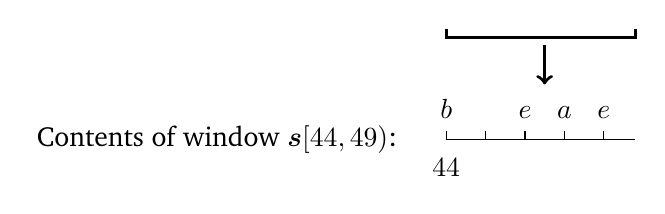
\begin{tikzpicture}

\examplesequence
\examplesequencetimestamps

\draw [very thick] (1.5,-0.6) -- ++(0,-3pt) -- ++(2.4,0) -- ++(0,3pt);

\draw [->,very thick] (2.75,-0.8) -- ++(0,-0.5);

\draw (1.5,-2) -- ++(2.4,0);

\foreach \x in {1.5,2,...,3.5}
    \draw (\x,-2) -- ++(0,3pt);

\foreach \x/\label in {
    1.5/b,
    2.5/e,
    3/a,
    3.5/e}
    \path (\x,-2) ++(0,1em) node [enoughdamnvspace] {$ \label $};

\path (1.5,-2) ++(0,-1em) node {$ 44 $};

\node [anchor=east] at (1,-2) {Contents of window $ \boldsymbol{s}[44,49) $:};

\end{tikzpicture}

\caption{A window of width 5 on a sequence $ \boldsymbol{s} $.}
\label{fig:windows}
\end{figure}

\subsection{Episodes}

Now we formally define patterns.

\begin{definition}
An \emph{episode} $ \alpha $ is a directed acyclic graph with labelled nodes, that is, $ \alpha = (V, E, lab) $, where $ V = (v_1, \ldots, v_k) $ is the set of nodes, $ E $ is the set of directed edges, and \emph{lab} is a function $ lab \colon V \rightarrow \Sigma $, mapping each node $ v_i $ to an event type. If $ lab(v) = A $, then we say that node $ v $ is of (event) type $ A $, and that $ \alpha $ contains $ A $, or $ A $ is in $ \alpha $.
\end{definition}

We write $ | \alpha | $ to mean the number of nodes in an episode's graph. We call $ | \alpha | $ the \emph{size} of $ \alpha $.

\begin{definition}
A node $ n $ in an episode graph is a \emph{descendant} of a node $ m $ if there is a path from $ m $ to $ n $. Conversely $ m $ is an \emph{ancestor} of $ n $ in that case.
\end{definition}

\begin{definition}
Given a sequence $ \boldsymbol{s} $ and an episode $ \alpha $ we say that $ s $ \emph{covers} $ \alpha $, or $ \alpha $ \emph{occurs in} $ \boldsymbol{s} $, if there is an injective map $ f $ mapping each node $ v_i $ to a valid index such that:
\begin{enumerate}
\item the node $ v_i $ in $ \alpha $ and the corresponding sequence element $ \boldsymbol{s}_{f(v_i)} $ are of the same event type: $ \boldsymbol{s}_{f(v_i)} = lab(v_i) $, and
\item if there is an edge $ (v_i, v_j) $ in $ \alpha $, then we must have $ f(v_i) < f(v_j) $. In other words, the parents of $ v_j $ must occur in $ \boldsymbol{s} $ before $ v_j $. If the mapping $ f $ is surjective, that is, all events in $ \boldsymbol{s} $ are used, we will say that $ \boldsymbol{s} $ is an \emph{instance} of $ \alpha $.
\end{enumerate}
\end{definition}

\begin{definition}
Episodes $ \alpha $ and $ \beta $ are said to be \emph{equivalent} if each sequence that covers $ \alpha $ also covers $ \beta $, and vice versa.
\end{definition}

In this thesis, we'll be limiting ourselves to two subcategories of episodes:
\begin{itemize}
\item \textbf{Parallel episodes.} A parallel episode is an episode for which the set of edges is empty. As such, no constraints are placed on the order in which event types occur in a sequence. An example is shown in figure~\ref{fig:episode-graphs-parallel}. In text we'll write parallel episodes by their event types using the following notation:
\begin{align*}
    \{ A_1, A_2, \ldots, A_n \}
\end{align*}
by which we mean a parallel episode with $ n $ nodes, and the event types are $ A_1 $ through $ A_n $. Note that though the notation reminds strongly of the notation for a mathematical set, it does not actually represent a set: a parallel episode $ \{ a, a, b, c \} $ is not equivalent to an episode $ \{ a, b, c \} $.

\item \textbf{Serial episodes.} A serial episode is an episode for which the edges cause the nodes to have a total order. That way, in any occurrence of a serial episode in a sequence, the event types appear in the same order. Figure~\ref{fig:episode-graphs-serial} shows an example.

% Sometimes it is useful to describe serial episodes in their strict form, in which there is a direct edge between any two nodes. Figure~\ref{fig:episode-graphs-serial-strict} shows a strict episode which is equivalent to the episode in figure~\ref{fig:episode-graphs-serial}.

While serial episodes have a different graph in this form, their meaning is the same, since they enforce the same order on the occurrence of events in the sequence to satisfy an occurrence of a serial episode.

For serial episodes we will use the notation
\begin{align*}
    A_1 \to A_2 \to \cdots \to A_n
\end{align*}
where $ A_i $ is the event type of the $ i $-th node, and a node of event type $ A_i $ is an ancestor of a node of event type $ A_j $ if $ i < j $.

\end{itemize}

\begin{figure}

\begin{subfigure}[b]{\textwidth}
\centering
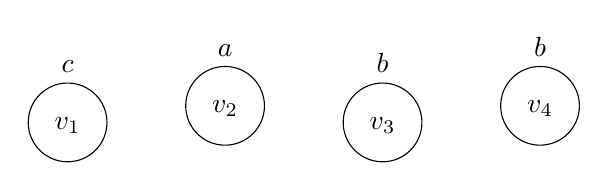
\begin{tikzpicture}

\node (n 1) [circly,label={$ c $},enoughdamnvspace] at (-3,-3pt) {$ v_1 $};
\node (n 2) [circly,label={$ a $},enoughdamnvspace] at (-1, 3pt) {$ v_2 $};
\node (n 3) [circly,label={$ b $},enoughdamnvspace] at ( 1,-3pt) {$ v_3 $};
\node (n 4) [circly,label={$ b $},enoughdamnvspace] at ( 3, 3pt) {$ v_4 $};

\end{tikzpicture}
\caption{parallel}
\label{fig:episode-graphs-parallel}
\end{subfigure}

\par\bigskip

\begin{subfigure}[b]{\textwidth}
\centering
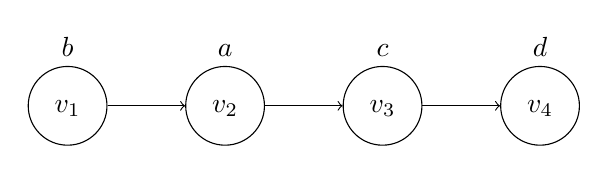
\begin{tikzpicture}

\node (n 1) [circly,label={$ b $},enoughdamnvspace] at (-3,0) {$ v_1 $};
\node (n 2) [circly,label={$ a $},enoughdamnvspace] at (-1,0) {$ v_2 $};
\node (n 3) [circly,label={$ c $},enoughdamnvspace] at ( 1,0) {$ v_3 $};
\node (n 4) [circly,label={$ d $},enoughdamnvspace] at ( 3,0) {$ v_4 $};

\draw [->] (n 1) -- (n 2);
\draw [->] (n 2) -- (n 3);
\draw [->] (n 3) -- (n 4);

\end{tikzpicture}
\caption{serial}
\label{fig:episode-graphs-serial}
\end{subfigure}

\par\bigskip

\iffalse
\begin{subfigure}[b]{\textwidth}
\centering
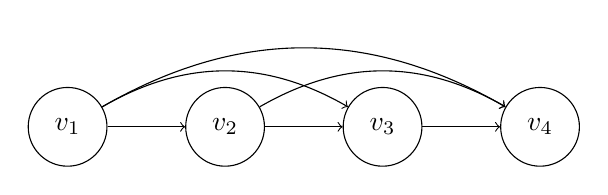
\begin{tikzpicture}

\node (n 1) [circly] at (-3,0) {$ v_1 $};
\node (n 2) [circly] at (-1,0) {$ v_2 $};
\node (n 3) [circly] at ( 1,0) {$ v_3 $};
\node (n 4) [circly] at ( 3,0) {$ v_4 $};

\draw [->] (n 1) -- (n 2);
\draw [->] (n 2) -- (n 3);
\draw [->] (n 3) -- (n 4);

\draw [->] (n 1) to [bend left=30] (n 3);
\draw [->] (n 2) to [bend left=30] (n 4);
\draw [->] (n 1) to [bend left=30] (n 4);

\end{tikzpicture}

\caption{serial, strict}
\label{fig:episode-graphs-serial-strict}
\end{subfigure}
\fi

\caption{An example of an episode graph for each of the episode class we will consider, with the event types shown above the nodes.}

\label{fig:episode-graphs}
\end{figure}

\begin{figure}
\centering

\begin{tikzpicture}

\examplesequence
\examplesequencetimestamps

\foreach \x [evaluate=\x as \timestamp using int((\x*2)+41)] in {-5.5,-5,...,5.5}
    \node (t\timestamp) [inner sep=0] at (\x,1.8em) {};

% serial episode

\node (serC) at (-5,2.5) [smallnode,label={$ c $}] {};
\node (serF) at (-4,2.5) [smallnode,label={$ f $}] {};
\node (serB) at (-3,2.5) [smallnode,label={$ b $}] {};

\draw [->,very thick] (serC) -- (serF);
\draw [->,very thick] (serF) -- (serB);

\draw [->] ([yshift=-3pt]serC.south) .. controls +(0,-1) and +(0,1) .. (t32);
\draw [->] ([yshift=-3pt]serF.south) .. controls +(0,-1) and +(0,1) .. (t33);
\draw [->] ([yshift=-3pt]serB.south) .. controls +(0,-1) and +(0,1) .. (t34);

% parallel episode

\node (parB) at (3,2.6) [smallnode,label={$ b $}] {};
\node (parE1) at (2,1.8) [smallnode,label={$ e $}] {};
\node (parE2) at (4.5,2.4) [smallnode,label={$ e $}] {};
\node (parC) at (3.5,2) [smallnode,label={$ c $}] {};

\draw [->] ([yshift=-3pt]parB.south) .. controls +(0,-1) and +(0,1) .. (t44);
\draw [->] ([yshift=-3pt]parE1.south) .. controls +(0,-0.5) and +(0,0.5) .. (t46);
\draw [->] ([yshift=-3pt]parE2.south) .. controls +(0,-1) and +(0,1) .. (t48);
\draw [->] ([yshift=-3pt]parC.south) .. controls +(0,-0.5) and +(0,0.5) .. (t49);

\end{tikzpicture}

\caption{Showing an occurrence of a serial episode $ c \to f \to b $ and an occurrence of a parallel episode $ \{ b, c, e, e \} $ in the sequence of figure~\ref{fig:event-sequence}.}
\label{fig:occurrences}
\end{figure}

Because we only consider parallel and serial episodes, it is easy to represent an episode in a data structure---we don't need to explicitly store a graph with nodes and edges:
\begin{itemize}
\item Parallel episodes can be stored in an array, where each element is simply the event type of the episode. Strictly speaking, the order of the elements in the array doesn't matter, but it can be useful for them to follow some order on the set of event types. In that way each parallel episode has a unique array representation. Figure~\ref{fig:parallel-representation} shows the representation visually.

\tikzset{circly/.style={draw,circle,minimum size=1cm},
    arraycell/.style={draw,rectangle,minimum size=1cm,node distance=0}}

\begin{figure}[h]
\centering

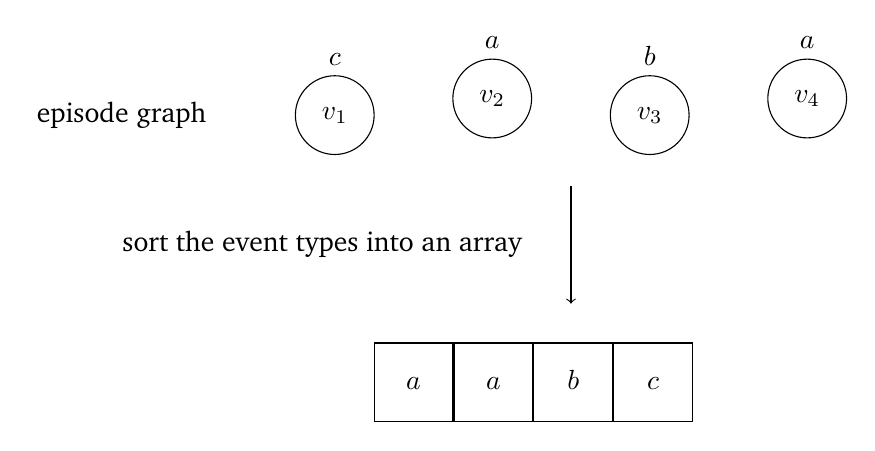
\begin{tikzpicture}

\node (n 1) [circly,label=above:$ c $] at (-3,-3pt) {$ v_1 $};
\node (n 2) [circly,label=above:$ a $] at (-1, 3pt) {$ v_2 $};
\node (n 3) [circly,label=above:$ b $] at ( 1,-3pt) {$ v_3 $};
\node (n 4) [circly,label=above:$ a $] at ( 3, 3pt) {$ v_4 $};

\node [left=of n 1] {episode graph};

\draw [->] (0,-1) -- node [left=0.5cm] {sort the event types into an array} +(0,-1.5);

\node (a 1) [arraycell,enoughdamnvspace] at (-2,-3.5) {$ a $};
\node (a 2) [arraycell,right=of a 1,enoughdamnvspace] {$ a $};
\node (a 3) [arraycell,right=of a 2,enoughdamnvspace] {$ b $};
\node (a 4) [arraycell,right=of a 3,enoughdamnvspace] {$ c $};

\end{tikzpicture}

\caption{A parallel episode's graph representation, with the label of each node shown above, and its array representation.}

\label{fig:parallel-representation}
\end{figure}

\item Serial episodes can also be stored in an array, but here the order of the elements is defined by the edges of the episode. That is, the event types are ordered according to a topological sort of the nodes. Figure~\ref{fig:serial-representation} shows this visually.
\end{itemize}

\begin{figure}[h]
\centering

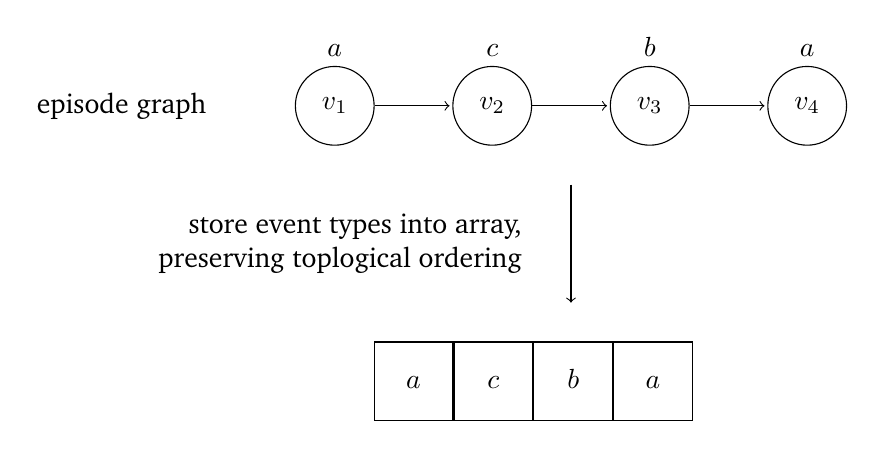
\begin{tikzpicture}

\node (n 1) [circly,label=above:$ a $] at (-3,0) {$ v_1 $};
\node (n 2) [circly,label=above:$ c $] at (-1,0) {$ v_2 $}
    edge [pre] (n 1);
\node (n 3) [circly,label=above:$ b $] at (1, 0) {$ v_3 $}
    edge [pre] (n 2);
\node (n 4) [circly,label=above:$ a $] at (3, 0) {$ v_4 $}
    edge [pre] (n 3);

\node [left=of n 1] {episode graph};

\draw [->] (0,-1) -- node [left=0.5cm,align=right] {store event types into array,\\preserving toplogical ordering} +(0,-1.5);

\node (a 1) [arraycell,enoughdamnvspace] at (-2, -3.5) {$ a $};
\node (a 2) [arraycell,right=of a 1,enoughdamnvspace] {$ c $};
\node (a 3) [arraycell,right=of a 2,enoughdamnvspace] {$ b $};
\node (a 4) [arraycell,right=of a 3,enoughdamnvspace] {$ a $};

\end{tikzpicture}

\caption{A serial episode's graph representation, with the label of each node shown above, and its array representation.}
\label{fig:serial-representation}
\end{figure}

When discussing the algorithms we will mostly consider their array representation, and address the $ i $-th element of an episode array $ \alpha $ with $ \alpha [i] $.

\begin{definition}
Given two episodes $ \alpha $ and $ \beta $, we say that $ \alpha $ is a \emph{subepisode} of $ \beta $, denoted $ \alpha \subseteq \beta $, if the set of all sequences that cover $ \beta $ is a subset of the set of all sequences that cover $ \alpha $. $ \alpha $ is a \emph{proper subepisode} of $ \beta $ if $ \alpha \subseteq \beta $ and $ \alpha $ and $ \beta $ are not equivalent. In that case we can write $ \alpha \subset \beta $.
\end{definition}

Of course, considering all event sequences that cover an episode is an impossible task, so the above definition does not give rise to a practical way of determining whether one episode is a subepisode of another. Instead we must look at the episodes themselves, and reason about all of the ways in which they might occur in a sequence. For parallel and serial episodes, it is quite straightforward to do so, as described below. More general cases have been reasoned about~\cite{tatti12}, but are beyond the scope of this thesis.

\begin{itemize}
\item A parallel episode $ \alpha $ is a subepisode of a parallel episode $ \beta $ if:
\begin{enumerate}
\item $ | V(\alpha) | \leq | V(\beta) | $, and
\item for each event type $ A $ in $ \alpha $, the number of nodes $ v $ in $ \alpha $ for which $ lab(v) = A $, is no greater than the number of nodes for which the same holds in $ \beta $.
\end{enumerate}
\item For serial episodes, the above is also a condition. Additionally, for each node $ v $ in $ \alpha $ of type $ A $ that is an ancestor of a node $ u $ of type $ B $, $ \beta $ must also have two nodes for which the node with event type $ A $ precedes the node with event type $ B $. Put more simply, the ordering of event types must be preserved.
\end{itemize}

\begin{definition}
Given two episodes $ \alpha $ and $ \beta $ such that $ \beta \subset \alpha $, we can express an \emph{association rule} $ \alpha \Rightarrow \beta $. We call $ \alpha $ the \emph{head} of the rule, and $ \beta $ the \emph{tail} of the rule.
\end{definition}

Given an association rule $ \alpha \Rightarrow \beta $, we can define a confidence value $ c(\alpha \Rightarrow \beta) $, which expresses the likelihood of finding an occurrence of $ \beta $, given that we have an occurrence of $ \alpha $ in a sequence. So, intuitively, the confidence value of an association rule gives an indication of how well an occurrence of the head of the rule ``predicts'' an occurrence of the tail.

\subsection{Interestingness measures}

Having discussed episodes occurring in event sequences, we would now like to be able to express how interesting an episode is in regard to a sequence.

Traditionally, the most common interpretation of \emph{interestingness} is frequency, which expresses how often an episode occurs in the sequence. The more often an episode occurs, the more interesting it is considered to be.

Exactly how the frequency of an episode in a sequence should be defined, is not immediately clear in sequential pattern mining. We will present three methods to measure the frequency of an episode and the confidence of an association rule. In a later section, we implement a mining algorithm based on them.

We'll also briefly discuss some interestingness measures that are not based on frequency.

\subsubsection{Fixed windows}

The first frequency measure we discuss was first proposed in~\cite{winepi97}, and is based on windows of a fixed length.

\begin{definition}
Given a window size $ \rho $ and a sequence $ \boldsymbol{s} $, we define the \emph{fixed-window frequency} of an episode $ \alpha $ in $ \boldsymbol{s} $, denoted $ fr_f(\alpha, \boldsymbol{s}) $, to be the number of windows of size $ \rho $ in $ \boldsymbol{s} $ covering the episode:
\begin{align*}
fr_f(\alpha, \boldsymbol{s}) = | \{ \boldsymbol{s}[i, i + \rho) \mid \boldsymbol{s}[i, i + \rho) \text{ covers } \alpha \} |
\end{align*}
\end{definition}

At first sight, counting the number of windows which cover the episode might seem a good approach---intuitively, if an episode occurs in many windows, then it must be frequent. However, upon closer inspection, the frequency values it produces are often counterintuitive, as they don't reflect very well how many occurrences there really are.

Figure~\ref{fig:fwi-example} shows all of the windows of size 8 that cover the episodes shown in figure~\ref{fig:occurrences}. We observe that $ fr_f(\{ a, a, b, c \}) = 6 $, and $ fr_f(c \to f \to b) = 3 $. We can immediately see a drawback to this definition of frequency: the frequency values are highly dependent on the window size. If we were to choose a window size of $ 6 $ instead, then $ fr_f(\{ a, a, b, c \}) = 6 $ and $ fr_f(c \to f \to b) = 1 $. We also see that the more an occurrence is spread out, the fewer windows cover it, and consequently the lower the frequency will be.

\begin{figure}
\centering

\begin{tikzpicture}

\examplesequence

\foreach \x [evaluate=\x as \timestamp using int((\x*2)+41)] in {-5.5,-5,...,5.5}
    \node (t\timestamp) [inner sep=0] at (\x,1.8em) {};

%% draw occurrence proofs again
% serial episode

\node (serC) at (-5,2.5) [smallnode,label={$ c $}] {};
\node (serF) at (-4,2.5) [smallnode,label={$ f $}] {};
\node (serB) at (-3,2.5) [smallnode,label={$ b $}] {};

\draw [->,very thick] (serC) -- (serF);
\draw [->,very thick] (serF) -- (serB);

\draw [->] ([yshift=-3pt]serC.south) .. controls +(0,-1) and +(0,1) .. (t32);
\draw [->] ([yshift=-3pt]serF.south) .. controls +(0,-1) and +(0,1) .. (t33);
\draw [->] ([yshift=-3pt]serB.south) .. controls +(0,-1) and +(0,1) .. (t34);

% parallel episode

\node (parB) at (3,2.6) [smallnode,label={$ b $}] {};
\node (parE1) at (2,1.8) [smallnode,label={$ e $}] {};
\node (parE2) at (4.5,2.4) [smallnode,label={$ e $}] {};
\node (parC) at (3.5,2) [smallnode,label={$ c $}] {};

\draw [->] ([yshift=-3pt]parB.south) .. controls +(0,-1) and +(0,1) .. (t44);
\draw [->] ([yshift=-3pt]parE1.south) .. controls +(0,-0.5) and +(0,0.5) .. (t46);
\draw [->] ([yshift=-3pt]parE2.south) .. controls +(0,-1) and +(0,1) .. (t48);
\draw [->] ([yshift=-3pt]parC.south) .. controls +(0,-0.5) and +(0,0.5) .. (t49);

% windows

\newcommand{\windowthingy}[1]
{
    \draw #1 -- ++(0,-3pt) -- ++(3.9,0) -- ++(0,3pt);
}

\windowthingy{(-7,-5pt)}
\windowthingy{(-6.5,-10pt)}
\windowthingy{(-6,-15pt)}
\windowthingy{(-5.5,-20pt)}
\windowthingy{(-5,-25pt)}
\windowthingy{(-4.5,-30pt)}

\windowthingy{(0.5,-5pt)}
\windowthingy{(1,-10pt)}
\windowthingy{(1.5,-15pt)}

\end{tikzpicture}

\caption{All of the windows of size 8 that cover two episodes in a sequence; a parallel episode $ \{a, a, b, c \} $ and a serial episode $ c \to f \to b $.}
\label{fig:fwi-example}
\end{figure}

\begin{definition}
Given a window size $ \rho $ and episodes $ \alpha $ and $ \beta $, such that $ \alpha \subset \beta $, we define the \emph{fixed-window confidence} of the association rule $ \alpha \Rightarrow \beta $, denoted $ c_f(\alpha \Rightarrow \beta) $, to be the ratio of their respective frequencies:
\begin{align*}
c_f(\alpha \Rightarrow \beta) = \frac{ fr_f(\beta) }{ fr_f(\alpha) }
\end{align*}
\end{definition}

Given that the fixed-window frequency gave unintuitive results for episodes, and that the fixed-window confidence is based on the fixed-window frequency, it should be no surprise that the confidence values for the fixed-window confidence can also be unintuitive.

Consider again the occurrence of the parallel episode in figure~\ref{fig:fwi-assoc-example}. With $ \rho = 8 $ as in the figure, $ fr_f(\{ e, e \}) = 6 $.

\begin{figure}
\centering

\begin{tikzpicture}

\clip (0,-10) rectangle (10,10);

\examplesequence

\foreach \x [evaluate=\x as \timestamp using int((\x*2)+41)] in {-5.5,-5,...,5.5}
    \node (t\timestamp) [inner sep=0] at (\x,1.8em) {};

%% draw occurrence proofs again
% serial episode

\node (serC) at (-5,2.5) [smallnode,label={$ c $}] {};
\node (serF) at (-4,2.5) [smallnode,label={$ f $}] {};
\node (serB) at (-3,2.5) [smallnode,label={$ b $}] {};

\draw [->,very thick] (serC) -- (serF);
\draw [->,very thick] (serF) -- (serB);

\draw [->] ([yshift=-3pt]serC.south) .. controls +(0,-1) and +(0,1) .. (t32);
\draw [->] ([yshift=-3pt]serF.south) .. controls +(0,-1) and +(0,1) .. (t33);
\draw [->] ([yshift=-3pt]serB.south) .. controls +(0,-1) and +(0,1) .. (t34);

% parallel episode

\node (parB) at (3,2.6) [smallnode,label={$ b $}] {};
\node (parE1) at (2,1.8) [smallnode,label={$ e $}] {};
\node (parE2) at (4.5,2.4) [smallnode,label={$ e $}] {};
\node (parC) at (3.5,2) [smallnode,label={$ c $}] {};

\draw [->] ([yshift=-3pt]parB.south) .. controls +(0,-1) and +(0,1) .. (t44);
\draw [->] ([yshift=-3pt]parE1.south) .. controls +(0,-0.5) and +(0,0.5) .. (t46);
\draw [->] ([yshift=-3pt]parE2.south) .. controls +(0,-1) and +(0,1) .. (t48);
\draw [->] ([yshift=-3pt]parC.south) .. controls +(0,-0.5) and +(0,0.5) .. (t49);

% windows

\newcommand{\windowthingy}[1]
{
    \draw #1 -- ++(0,-3pt) -- ++(3.9,0) -- ++(0,3pt);
}

\windowthingy{(-7,-5pt)}
\windowthingy{(-6.5,-10pt)}
\windowthingy{(-6,-15pt)}
\windowthingy{(-5.5,-20pt)}
\windowthingy{(-5,-25pt)}
\windowthingy{(-4.5,-30pt)}

\windowthingy{(0.5,-5pt)}
\windowthingy{(1,-10pt)}
\windowthingy{(1.5,-15pt)}

\end{tikzpicture}

\label{fig:fwi-assoc-example}
\end{figure}

\subsubsection{Minimal windows}

\begin{definition}
Given a sequence $ s $ and an episode $ G $, a window $ s[a, b] $, is called a \emph{minimal window} of $ G $ in $ s $, if:
\begin{itemize}
\item $ len(s[a, b]) \leq \rho $, $ s[a, b] $, and
\item no proper subwindow of of $ s[a, b] $ covers $ G $.
\end{itemize}
We define beginning, end ... % TODO figure out definitions (inclusive-exclusive end-timestamp)

We denote the set of all minimal windows of $ G $ in $ s $ with $ mw(G; s) $, or simply $ mw(G) $ if $ s $ is known from the context. Given a set of minimal windows $ W $, we define a function $ dis(W) $ to be equal to 1 if all windows in $ W $ are pairwise disjoint, and 0 otherwise.
\end{definition}

\begin{definition}
The \emph{disjoint-window frequency} of an episode $ G $ in a sequence $ s $, denoted $ fr_m(G) $, is defined as the maximal number of non-overlapping minimal windows within $ s $ that contain episode $ G $. Formally:
\begin{align*}
fr_m(G) = \text{max} \{ | W | \mid W \subseteq mw(G) \wedge dis(W) = 1 \}
\end{align*}
\end{definition}

\begin{definition}
Given episodes $ X $ and $ Y $, such that $ X \subset Y $, and a minimal window $ s[a, b] $ of episode $ X $. Assume there exists a minimal window $ s[c, d] $ of $ Y $ such that $ c \leq a $ and $ b \leq d $, then we define the \emph{minimal-extensibility} of occurrence $ s[a, b] $ of $ X $ into an occurrence of $ Y $ as
\begin{align*}
ext_m(s[a, b], X, Y) = 1
\end{align*}
If there exists no such minimal window of $ Y $, we define $ ext_m(s[a, b], X, Y) = 0 $.
\end{definition}

\subsubsection{Weighted minimal windows}

\begin{definition}
The \emph{total weight} of a set of windows $ W $ in a sequence $ s $, denoted $ tw(W) $, is defined as
\begin{align*}
tw(W) = \sum_{w \in W}{\frac{1}{len(w)}}
\end{align*}
The \emph{weighted-window frequency} of an episode $ G $ in a sequence $ s $, denoted $ fr_w(G) $, is defined as
\begin{align*}
fr_w(G) = \text{max} \{ tw(W) | W \subseteq mw(G), dis(W) = 1 \}
\end{align*}
\end{definition}

\subsubsection{Other interestingness measures}

\newpage

\section{Algorithms}

\begin{algorithm}

\caption{Recognizing serial episodes using the fixed-window frequency measure. \\
Input: A collection $ \mathcal{C} $ of serial episodes, an event sequence $ \boldsymbol{s} = (s, T_s, T_e) $, a window width \textit{win}, and a frequency threshold \textit{min\_fr}. \\
Ouptut: The episodes of $ \mathcal{C} $ that are frequent in $ \boldsymbol{s} $ with respect to \textit{win} and \textit{min\_fr}.
}

\begin{algorithmic}[1]

\ForAll{$ \alpha \in \mathcal{C} $}
    \For{$ i \leftarrow 1 $ to $ | \alpha | $}
        \State{$ \alpha \text{.initialized} \leftarrow 0 $}
        \State{$ \text{waits}(\alpha[i]) \leftarrow 0 $}
    \EndFor
\EndFor

\ForAll{$ \alpha \in \mathcal{C} $}
    \State{$ \text{waits}(\alpha[1]) \leftarrow \text{waits}(\alpha[1]) \cup \left\{ \left( \alpha, 1 \right) \right\} $}
    \State{$ \alpha \text{.freq\_count} \leftarrow 0 $}
\EndFor

\For{$ t \leftarrow T_s - \text{win} $ to $ T_s - 1 $}
    \State{$ \text{begins\_at}(t) \leftarrow \emptyset $}
\EndFor

\For{$ \text{start} \leftarrow T_s - \text{win} + 1 $ to $ T_e $}
    \State{$ \text{begins\_at}(\text{start} + \text{win} - 1) \leftarrow \emptyset $}
    \State{$ \text{transitions} \leftarrow \emptyset $}
    \ForAll{events $ (A, t) $ in $ s $ such that $ t = \text{start} + \text{win} - 1 $}
        \ForAll{$ ( \alpha, j) \in \text{waits}(A) $}
            \If{$ j = | \alpha | $ and $ \alpha \text{.initialized}[j] = 0 $}
                \State{$ \alpha \text{.in\_window} \leftarrow \text{start} $}
            \EndIf
            \If{$ j = 1 $}
                \State{$ \text{transitions} \leftarrow \text{transitions} \cup \{ ( \alpha, 1, \text{start} + \text{win} - 1 ) \} $}
            \Else
                \State{$ \text{transitions} \leftarrow \text{transitions} \cup \{ \alpha, j, \alpha \text{.initialized} [j - 1] \} $}
                \State{$ \text{begins\_at}( \alpha \text{.initialized}[j - 1] ) \leftarrow $
                \State \hspace{\algorithmicindent} $ \text{begins\_at}( \alpha \text{.initialized}[j - 1] ) \setminus \{ ( \alpha, j - 1 ) \} $}
                \State{$ \alpha \text{.initialized} [j - 1] \leftarrow 0 $}
                \State{$ \text{waits}(A) \leftarrow \text{waits}(A) \setminus \{ ( \alpha, j ) \} $}
            \EndIf
        \EndFor
    \EndFor
    \ForAll{$ ( \alpha, j, t ) \in \text{transitions} $}
        \State{$ \alpha \text{.initialized} [j] \leftarrow t $} \label{alglin:rec-ser-fwi:transition-begin}
        \State{$ \text{begins\_at}(t) \leftarrow \text{begins\_at}(t) \cup \{ ( \alpha, j ) \} $}
        \If{$ j < | \alpha | $}
            \State{$ \text{waits}(\alpha [j + 1]) \leftarrow \text{waits}(\alpha [j + 1]) \cup \{ (\alpha, j + 1) \} $} \label{alglin:rec-ser-fwi:transition-end}
        \EndIf
    \EndFor
    \ForAll{$ (\alpha, l) \in \text{begins\_at}(\text{start} - 1) $}
        \If{$ l = | \alpha | $} \label{alglin:rec-ser-fwi:cleanup-begin}
            \State{$ \alpha \text{.freq\_count} \leftarrow \alpha \text{.freq\_count} - \alpha \text{.in\_window} + \text{start} $}
        \Else
            \State{$ \text{waits}(\alpha [l + 1]) \leftarrow \text{waits}(\alpha [l + 1]) \setminus \{ ( \alpha, l + 1 ) \} $}
        \EndIf
        \State{$ \alpha \text{.initialized}[l] \leftarrow 0 $} \label{alglin:rec-ser-fwi:cleanup-end}
    \EndFor
\EndFor
\ForAll{episodes $ \alpha $ in $ \mathcal{C} $}
    \If{$ \alpha \text{.freq\_count} / T_e - T_s + \text{win} - 1 \geq \text{min\_fr} $}
        \State{output $ \alpha $}
    \EndIf
\EndFor

\end{algorithmic}

\label{alg:rec-ser-fwi}
\end{algorithm}

Algorithm~\ref{alg:rec-ser-fwi} is for recognizing a collection of episodes $ \mathcal{C} $ in a sequence. By the definition of serial episodes, all nodes must appear in the sequence in a strict order. Serial episodes are therefore recognized using automata, instances of which advance as events are encountered. The algorithm iterates over the sequence once.

Each episode has its own automaton, which consists of $ | \alpha | $ states: each state corresponds to a node in the episode. A state can be represented by the array index in the episode it corresponds to; 1 referring to the first node in the topological ordering of the episode graph, and so on. Then an instance of the automaton for $ \alpha $ being in a state $ j $ denotes that the episode has been recognized up to (and including) the $ j $-th node. When in state $ j $ and upon encountering an event of which the type corresponds to the type of the $ (j + 1) $-th node of the episode, the instance will transition to state $ j + 1 $.

When an instance of $ \alpha $ reaches state $ | \alpha | $, the episode has been successfully recognized, and as the iteration over the sequence continues, the number of windows which cover the instance of the episode get counted.

If the timestamp at which the automaton instance was initialized falls out of the window before reaching state $ | \alpha | $, the instance is removed.

The algorithm uses some bookkeeping data structures, which get updated as the sequence gets read. We'll discuss the most important ones.
\begin{itemize}
\item \textbf{waits} maps an event type to a set of pairs of the form $ (\alpha, j) $, where $ \alpha $ is an episode and $ j $ represents a state in the episode's automaton. If a pair $ (\alpha, j) $ is in $ waits(A) $, then $ \alpha $ has an instance of its automaton currently in state $ (j - 1) $ and is waiting for an event of type $ A $ to advance to the next state. Throughout the iteration over the sequence, $ \text{waits}(A) $ will always contain $ (\alpha, 1) $ for each episode $ \alpha $ that starts with $ A $, since it's always waiting to start a new instance of its automaton.
\item \textbf{begins\_at} maps a timestamp to a set of pairs $ (\alpha, j) $. If $ (\alpha, j) $ is in $ \text{begins}\_at(t) $, then $ \alpha $ has an instance of its automaton in state $ j $, and the automaton first entered this state at timestamp $ t $.
\item Each episode $ \alpha $ has an $ | \alpha | $-element array called \textbf{initialized}, which maps each of its automaton's states to the timestamp in the sequence at which the instance currently in that state was initialized. If for a certain state there is currently no active instance, its corresponding element in the initialized array will be some special value---[Winepi] chose 0, which we changed to UNINITIALIZED for clarity and such that 0 can be a valid timestamp if necessary.

This approach works because there never needs to be more than one automaton instance per state. If one automaton instance reaches the current state of another instance, they will simply make transitions simultaneously until the earlier instance gets removed. It suffices to maintain the instance which was reached the common state last, since it was initialized at a later timestamp, and thus will be the last to be removed.
\end{itemize}

While implementing this algorithm we found an error in the pseudocode, related to multiple instances of an episode's automaton reaching a common state. At line~\ref{alglin:rec-ser-fwi:transition-begin}, a transition of an automaton instance is being applied. The \emph{initialized} array gets updated, potentially overwriting a previous instance in the same state. \emph{begins\_at} gets updated with the new state, but the information about the potentially overwritten instance is not removed from \emph{begins\_at}. We'll illustrate how this affects the output with an example.

Using a window width of 2, and scanning the subsequence $ \cdots E \: A \: E \: C \cdots $. (This sequence of events appears in figure 2 in [Winepi].) Say that the first $ E $ has timestamp $ t_1 $. Consider the recognition of the serial episode $ \alpha = E \to C $. Obviously the subsequence contains the episode, and a window width of 2 suffices to recognize an instance of the episode in the subsequence. Upon encountering the first $ E $, an automaton instance gets initialized for $ \alpha $, as shown in lines \ref{alglin:rec-ser-fwi:transition-begin} through \ref{alglin:rec-ser-fwi:transition-end}. This includes:
\begin{itemize}
\item setting the timestamp in the \emph{initialized} array;
\item adding $ (\alpha, 2) $ to the $ \text{waits}(C) $ set (so that if $ C $ is encountered, the automaton can transition to the next state);
\item adding $ (\alpha, 1) $ to $ \text{begins\_at}(t_1) $ (to facilitate the removal of the the automaton instance once $ t $ falls out of the window).
\end{itemize}

When the second $ E $ is read (at $ t = t_1 + 2 $ and when $ \text{start} = t_1 + 1 $), a new instance of the automaton is created, and since the previous instance is still in state $ 1 $---no $ C $ has been encountered---the previous instance must be removed. However, $ (\alpha, 1) $ remains in $ \text{begins\_at}(t_1) $. Just after, this newly created automaton is wrongly removed (lines \ref{alglin:rec-ser-fwi:cleanup-begin} through \ref{alglin:rec-ser-fwi:cleanup-end}) and $ \alpha $ fails to get recognized.

\newpage


\chapter{Experiments}
\label{sec:experiments}

A big point of comparison while implementing our algorithms was a closed episode miner\footnote{http://adrem.ua.ac.be/mining-closed-strict-episodes}. It allowed us to verify the correctness of our implementation. The closed episode miner differs in a few ways from our implementation:

\begin{itemize}
\item It generates general episodes, not just parallel and serial episodes.
\item It generates closed episodes. Closed episodes are episodes that have no superepisodes of the same frequency. Mining only closed episodes helps in reducing the amount of output. The implementation has options to mine non-closed episodes as well, though, which allows us to compare with our implementation.
\item While our implementation finds episodes of one class at a time, as specified by the user---parallel or serial---the closed episode miner finds episodes of all classes at once---parallel, serial and general.
\end{itemize}

Given the above, in order to compare the two implementations in terms of their output, we have to enable the options that cause the closed episode miner to find non-closed episodes, since our implementation finds non-closed episodes as well; and we have to filter out those episodes which don't match the class of episodes we're currently mining.

Mining general episodes is of higher complexity than parallel and serial episodes.

Parallel episodes can only ``grow'' by adding a new node, and serial episodes grow in much the same way: by adding a node and an edge at the same time. Pattern explosion is a bigger concern with general episodes: additionally, they can grow by adding only an edge. So, ideally, our implementation should be faster than the closed episode miner.

% ^ terrible ^

\section{Datasets}

We will conduct experiments using a number of datasets:

\begin{itemize}
\item \emph{abstract}: a dataset consisting of the first 739 NSF award abstracts from 1990, merged into one long sequence\footnote{\url{http://kdd.ics.uci.edu/databases/nsfabs/nsfawards.html}}.
\item \emph{tolstoy}: Leo Tolstoy's novel Anna Karenina, from Project Gutenberg\footnote{\url{https://www.gutenberg.org/ebooks/1399}}.
\item \emph{trains}: a dataset consisting of departure times of delayed trains in a Belgian railway station, for trains with a delay of at least three minutes. This data is anonymized, so we won't be able derive any meaning from the patterns, but it it an interesting dataset nonetheless, because contrary to the textual datasets, \emph{trains} is sparse.
\end{itemize}

The textual datasets were preprocessed by lemmatizing using the Porter stemmer\footnote{\url{https://tartarus.org/martin/PorterStemmer}} and stop words were removed.

Table~\ref{table:datasets-numbers} shows some statistics about each dataset, where $ | \Sigma | $ is the size of the alphabet, $ | s | $ is the number of events, and $ T_e - T_s $ is the time range of the sequence. For dense sequences, $ T_e - T_s = | s | $. For sparse sequences, a window of $ \rho $ contains on average $ | s | \frac\rho{T_e - T_s} $ events.

\begin{table}
\centering

\begin{tabulary}{\textwidth}{ L|RRRC }

dataset & \multicolumn{1}{c}{$ | \Sigma | $} & \multicolumn{1}{c}{$ | s | $} & \multicolumn{1}{c}{$ T_e - T_s $} & type \\
\hline
\emph{abstract} & $ 51\,346 $ & $ 67\,828 $ & $ 67\,828 $ & dense \\
\emph{tolstoy} & $ 95\,623 $ & $ 124\,627 $ & $ 124\,627 $ & dense \\
\emph{trains} & $ 7\,874 $ & $ 10\,115 $ & $ 26\,626\,667 $ & sparse \\

\end{tabulary}

\caption{Some properties of the datasets $ (s, T_s, T_e) $.}
\label{table:datasets-numbers}
\end{table}

We see that the textual and \emph{trains} datasets have quite large alphabets. Figures~\ref{fig:frequency-plot-nsf} and \ref{fig:frequency-plot-nsf} and \ref{fig:frequency-plot-tolstoy} show the number of occurrences of the most frequent event types, ordered by frequency. We observe a long tail\footnote{\url{https://en.wikipedia.org/wiki/Long_tail}} for \emph{abstract} and \emph{tolstoy}, which is common for natural-language texts. In \emph{trains}, too, there is a similar progression, with a small number of the event types occurring a significant number of times, and the vast majority of event types occurring very rarely. Note that the graphs don't even show all event types, although for \emph{abstract} and \emph{trains} the rightmost event types occur only once, and those for \emph{tolstoy} occur fewer than 10 times.

\begin{figure}
\centering

\def\testwidth{6cm}
\def\testheight{5cm}

\begin{subfigure}[b]{\textwidth}
\centering

\begin{tikzpicture}

\begin{axis}[
    width=\testwidth,
    height=\testheight,
    xlabel={event types ordered by frequency},
    ylabel={number of occurrences},
    % ymode=log
]

\addplot table [x=rank,y=count,mark=none] {experiments/nsf-alphabet-frequency-300.dat};

\end{axis}

\end{tikzpicture}

\caption{The frequency of the 300 most frequent events in \emph{abstract}.}
\label{fig:frequency-plot-nsf}
\end{subfigure}

\par\bigskip

\begin{subfigure}[b]{\textwidth}
\centering

\begin{tikzpicture}

\begin{axis}[
    width=\testwidth,
    height=\testheight,
    xlabel={event types ordered by frequency},
    ylabel={number of occurrences},
    % ymode=log
]

\addplot table [x=rank,y=count,mark=none] {experiments/tolstoy-alphabet-frequency-2200.dat};

\end{axis}

\end{tikzpicture}

\caption{The frequency of the 2200 most frequent events in \emph{tolstoy}.}
\label{fig:frequency-plot-tolstoy}
\end{subfigure}

\par\bigskip

\begin{subfigure}[b]{\textwidth}
\centering

\begin{tikzpicture}

\begin{axis}[
    width=\testwidth,
    height=\testheight,
    xlabel={event types ordered by frequency},
    ylabel={number of occurrences},
    % ymode=log
]

\addplot table [x=rank,y=count,mark=none] {experiments/trains-alphabet-frequency-300.dat};

\end{axis}

\end{tikzpicture}

\caption{The frequency of the 300 most frequent events in \emph{trains}.}
\label{fig:frequency-plot-trains}
\end{subfigure}

\caption{The frequency of the most frequent event types in the datasets.}
\label{fig:alphabet-frequencies}
\end{figure}


\section{Performance}
\label{sec:performance}

To assess the efficiency of the algorithm, we inspect the runtime for different input parameters: comparing both episode classes, the frequency measures, while varying the window width and the frequency and confidence thresholds.

The performance experiments were ran as follows. For specified episode classes, frequency measures, a list of window widths, and a range of frequency thresholds, an experiment would run the cartesian product of all these parameters, within time and memory constraints. A few particularities:

\begin{itemize}
\item The range of frequency thresholds has an exponentially decreasing nature: it is specified by a (high) starting threshold, a multiplier $ \in (0, 1) $, and a lower bound. Each iteration, the current frequency threshold is multiplied with the multiplier to obtain the next frequency threshold. For example, with a multiplier of 0.90, the next threshold is always 10\% smaller than the last.
\item For each combination of episode class, frequency measure, and window width, a thread is run with progressively lower frequency thresholds, as described above. If memory runs out or the timeout is exceeded before reaching the lower bound, all lower frequency thresholds for that combination of episode class, frequency measure, and window width are skipped, as they will take at least as much time and memory as the current threshold.
\end{itemize}

All performance experiments were run on the same machine; the full specifications of which can be found online\footnote{The specifications can be found at \url{https://support.apple.com/kb/sp623}. 2.7 GHz model; memory manually upgraded to 12~GB. Running macOS 10.13.5. All C++ code compiled with clang-900.0.39.2 from LLVM~9.0. All Java code run with Java~SE~1.8.}.


\subsection{Episodes}
\label{sec:performance-episodes}


\iffalse
% --- Plotting the number of candidates and the number of frequent episodes. Maybe not so useful.
\begin{tikzpicture}

\begin{axis}[
    legend entries={fixed windows,minimal windows,weighted windows},
    legend style={legend pos=outer north east},
    xlabel={number of candidates},
    ylabel={number of frequent episodes},
]

\addplot table [x=num-frequent-episodes,y=num-candidates] {experiments/nsf/nsf-parallel-fixed-windows-8.tsv};
\addplot table [x=num-frequent-episodes,y=num-candidates] {experiments/nsf/nsf-parallel-minimal-windows-8.tsv};
\addplot table [x=num-frequent-episodes,y=num-candidates] {experiments/nsf/nsf-parallel-weighted-windows-8.tsv};

\end{axis}

\end{tikzpicture}

\begin{tikzpicture}

\begin{axis}[
    legend entries={fixed windows,minimal windows,weighted windows},
    legend style={legend pos=outer north east},
    xlabel={number of candidates},
    ylabel={number of frequent episodes},
]

\addplot table [x=num-frequent-episodes,y=percentage-frequent-of-candidates] {experiments/nsf/nsf-parallel-fixed-windows-8.tsv};
\addplot table [x=num-frequent-episodes,y=percentage-frequent-of-candidates] {experiments/nsf/nsf-parallel-minimal-windows-8.tsv};
\addplot table [x=num-frequent-episodes,y=percentage-frequent-of-candidates] {experiments/nsf/nsf-parallel-weighted-windows-8.tsv};

\end{axis}

\end{tikzpicture}

\begin{tikzpicture}

\begin{axis}[
    legend entries={fixed windows,minimal windows,weighted windows},
    legend style={legend pos=outer north east},
    xlabel={number of candidates},
    ylabel={number of frequent episodes},
]

\addplot table [x=num-candidates,y=num-frequent-episodes] {experiments/trains/trains-parallel-fixed-windows-900.tsv};
\addplot table [x=num-candidates,y=num-frequent-episodes] {experiments/trains/trains-parallel-minimal-windows-900.tsv};
\addplot table [x=num-candidates,y=num-frequent-episodes] {experiments/trains/trains-parallel-weighted-windows-900.tsv};

\end{axis}

\end{tikzpicture}
% --- ---
\fi

\subsection{Association rules}

Figure~\ref{fig:runtimes-rules-trains-900} shows runtimes for generating association rules from \emph{trains} using different episode classes, as a function of the number of frequent episodes. Some weird results though % TODO fix

As we saw in algorithm~\ref{alg:association-rules-top-level}, for each frequent episode $ \beta $, all $ \alpha \Rightarrow \beta $ with $ \alpha \subset \beta $ are considered. In our experiments, the association mining process usually took a small fraction of the duration of the episode mining process. But, assuming an injective $ lab $-function (an event type appears at most once), the number of subepisodes of an episode is exponential in the size of the episode. So, when there was many large episodes, mining association rules started to take significant time.

\begin{figure}

\begin{subfigure}[b]{0.5\textwidth}
\centering

\begin{tikzpicture}[scale=0.65]

\begin{axis}[
    legend entries={fixed windows,minimal windows,weighted windows},
    legend style={legend pos=north west},
    xlabel={number of frequent episodes},
    ylabel={runtime (s)},
]

\addplot table [x=num-frequent-episodes,y=duration-rules-0.0] {experiments/nsf/nsf-parallel-fixed-windows-8.tsv};
\addplot table [x=num-frequent-episodes,y=duration-rules-0.0] {experiments/nsf/nsf-parallel-minimal-windows-8.tsv};
\addplot table [x=num-frequent-episodes,y=duration-rules-0.0] {experiments/nsf/nsf-parallel-weighted-windows-8.tsv};

\end{axis}

\end{tikzpicture}

\caption{rules consisting of parallel episodes}
\end{subfigure}
\begin{subfigure}[b]{0.5\textwidth}
\centering

\begin{tikzpicture}[scale=0.65]

\begin{axis}[
    legend entries={fixed windows,minimal windows,weighted windows},
    legend style={legend pos=north west},
    xlabel={number of frequent episodes},
    ylabel={runtime (s)},
]

\addplot table [x=num-frequent-episodes,y=duration-rules-0.0] {experiments/nsf/nsf-serial-fixed-windows-8.tsv};
\addplot table [x=num-frequent-episodes,y=duration-rules-0.0] {experiments/nsf/nsf-serial-minimal-windows-8.tsv};
\addplot table [x=num-frequent-episodes,y=duration-rules-0.0] {experiments/nsf/nsf-serial-weighted-windows-8.tsv};

\end{axis}

\end{tikzpicture}

\caption{rules consisting of serial episodes}
\end{subfigure}

\caption{Runtimes for finding association rules from episodes generated from \emph{trains} (same experiment as figure~\ref{fig:runtimes-trains-900}) for different confidence thresholds (0.0, 0.4 and 1.0).}
\label{fig:runtimes-rules-trains-900}
\end{figure}

\subsection{Number of candidate episodes versus number of frequent episodes}

The database passes are an expensive---if not the most expensive---part of the mining algorithm. Plotting the number of frequent episodes in the output and the number of candidates that were considered in a pass over the sequence gives us an idea of the amount of internal work the algorithms deal with for the output that gets produced.

\subsection{Comparing the frequency measures}

We would like to compare the efficiency for the different frequency measures across a range of frequency thresholds. However we should not evaluate the runtimes as a function of the frequency threshold directly, since the values for each of the measures are semantically different. For instance, the weighted-window frequency of an episode in a sequence is at most equal to the disjoint-window frequency; so for otherwise equal parameters (including thresholds), the weighted-window frequency will produce a subset of the disjoint-window frequency. Instead we can compare runtimes as a function of the number of frequent episodes.

Figure~\ref{fig:runtimes-nsf-8} shows such plots for both parallel and serial episodes, using the \emph{abstracts} dataset. We see that the fixed-window frequency performs significantly better than the other measures for parallel episodes. The weighted-window frequency runs up against the timeout very quickly in comparison.

For serial episodes, the fixed-window frequency has less of an advantage, and at a certain point the minimal-window frequency produces more episodes for in less time. This could be explained by the fact that the data pass algorithm that finds minimal windows of serial episodes is slightly simpler than the algorithm that determines the fixed-window frequency for serial episodes. While the weighted-window frequency algorithm uses the same data pass algorithms as the disjoint-window frequency, selecting the optimal selection of non-overlapping windows is more complex, explaining its higher runtimes.

\begin{figure}

\begin{subfigure}[b]{0.5\textwidth}
\centering

\begin{tikzpicture}[scale=0.65]

\begin{axis}[
    legend entries={fixed windows,minimal windows,weighted windows},
    legend style={legend pos=south east},
    xlabel={number of frequent episodes},
    ylabel={runtime (s)},
]

\addplot table [x=num-frequent-episodes,y=duration-s] {experiments/nsf/nsf-parallel-fixed-windows-8.tsv};
\addplot table [x=num-frequent-episodes,y=duration-s] {experiments/nsf/nsf-parallel-minimal-windows-8.tsv};
\addplot table [x=num-frequent-episodes,y=duration-s] {experiments/nsf/nsf-parallel-weighted-windows-8.tsv};

\end{axis}

\end{tikzpicture}

\caption{parallel episodes}
\end{subfigure}
\begin{subfigure}[b]{0.5\textwidth}
\centering

\begin{tikzpicture}[scale=0.65]

\begin{axis}[
    legend entries={fixed windows,minimal windows,weighted windows},
    legend style={legend pos=south east},
    xlabel={number of frequent episodes},
    ylabel={runtime (s)},
]

\addplot table [x=num-frequent-episodes,y=duration-s] {experiments/nsf/nsf-serial-fixed-windows-8.tsv};
\addplot table [x=num-frequent-episodes,y=duration-s] {experiments/nsf/nsf-serial-minimal-windows-8.tsv};
\addplot table [x=num-frequent-episodes,y=duration-s] {experiments/nsf/nsf-serial-weighted-windows-8.tsv};

\end{axis}

\end{tikzpicture}

\caption{serial episodes}
\end{subfigure}

\caption{Runtimes for finding episodes in dataset \emph{abstract} using a window width of 8.}
\label{fig:runtimes-nsf-8}
\end{figure}

\begin{figure}

\begin{subfigure}[b]{0.5\textwidth}
\centering

\begin{tikzpicture}[scale=0.65]

\begin{axis}[
    legend entries={fixed windows,minimal windows,weighted windows},
    legend style={legend pos=north west},
    xlabel={number of frequent episodes},
    ylabel={runtime (s)},
    xmode=log,
    ymode=log,
]

\addplot table [x=num-frequent-episodes,y=duration-s] {experiments/trains/trains-parallel-fixed-windows-900.tsv};
\addplot table [x=num-frequent-episodes,y=duration-s] {experiments/trains/trains-parallel-minimal-windows-900.tsv};
\addplot table [x=num-frequent-episodes,y=duration-s] {experiments/trains/trains-parallel-weighted-windows-900.tsv};

\end{axis}

\end{tikzpicture}

\caption{parallel episodes}
\end{subfigure}
\begin{subfigure}[b]{0.5\textwidth}
\centering

\begin{tikzpicture}[scale=0.65]

\begin{axis}[
    legend entries={fixed windows,minimal windows,weighted windows},
    legend style={legend pos=north west},
    xlabel={number of frequent episodes},
    ylabel={runtime (s)},
    xmode=log,
    ymode=log,
]

\addplot table [x=num-frequent-episodes,y=duration-s] {experiments/trains/trains-serial-fixed-windows-900.tsv};
\addplot table [x=num-frequent-episodes,y=duration-s] {experiments/trains/trains-serial-minimal-windows-900.tsv};
\addplot table [x=num-frequent-episodes,y=duration-s] {experiments/trains/trains-serial-weighted-windows-900.tsv};

\end{axis}

\end{tikzpicture}

\caption{serial episodes}
\end{subfigure}

\caption{Runtimes for finding episodes in dataset \emph{trains} using a window width of 8.}
\label{fig:runtimes-trains-900}
\end{figure}



\subsection{Comparing sequence lengths}

\begin{figure}

\begin{subfigure}[b]{0.5\textwidth}
\centering
\begin{tikzpicture}[scale=0.65]

\begin{axis}[
    legend pos=north west,
    legend entries={fixed windows,minimal windows,weighted windows},
    xlabel={portion of the whole sequence},
    ylabel={runtime (s)},
    % ymode=log,
]

\addplot table [x=portion,y=duration-s] {experiments/length/tolstoy-lengths-parallel-fixed-windows.dat};
\addplot table [x=portion,y=duration-s] {experiments/length/tolstoy-lengths-parallel-minimal-windows.dat};
\addplot table [x=portion,y=duration-s] {experiments/length/tolstoy-lengths-parallel-weighted-windows.dat};
% \addplot table [x=portion,y=duration-s] {experiments/length/tolstoy-lengths-serial-fixed-windows.dat};
% \addplot table [x=portion,y=duration-s] {experiments/length/tolstoy-lengths-serial-minimal-windows.dat};
% \addplot table [x=portion,y=duration-s] {experiments/length/tolstoy-lengths-serial-weighted-windows.dat};

\end{axis}

\end{tikzpicture}
\caption{linear scale}
\label{fig:tolstoy-runtime-vs-length-linear-scale}
\end{subfigure}
\begin{subfigure}[b]{0.5\textwidth}
\centering
\begin{tikzpicture}[scale=0.65]

\begin{axis}[
    legend pos=south east,
    legend entries={fixed windows,minimal windows,weighted windows},
    xlabel={portion of the whole sequence},
    ylabel={runtime (s)},
    ymode=log,
]

\addplot table [x=portion,y=duration-s] {experiments/length/tolstoy-lengths-parallel-fixed-windows.dat};
\addplot table [x=portion,y=duration-s] {experiments/length/tolstoy-lengths-parallel-minimal-windows.dat};
\addplot table [x=portion,y=duration-s] {experiments/length/tolstoy-lengths-parallel-weighted-windows.dat};
% \addplot table [x=portion,y=duration-s] {experiments/length/tolstoy-lengths-serial-fixed-windows.dat};
% \addplot table [x=portion,y=duration-s] {experiments/length/tolstoy-lengths-serial-minimal-windows.dat};
% \addplot table [x=portion,y=duration-s] {experiments/length/tolstoy-lengths-serial-weighted-windows.dat};

\end{axis}

\end{tikzpicture}
\caption{logaritmic scale}
\label{fig:tolstoy-runtime-vs-length-log-scale}
\end{subfigure}

\caption{Runtimes for different portions of \emph{tolstoy} using a fixed frequency threshold for each frequency measure. $ \rho = 15 $.}
\label{fig:tolstoy-runtime-vs-length}
\end{figure}

In sequential pattern mining, sequences are expected to be very long. Therefore we would like to have an idea of how the length of the sequence affects the performance. We measured the runtime of the algorithm for different-sized prefixes of the \emph{tolstoy} dataset for all episode classes and frequency measures. The results can be seen in figure~\ref{fig:tolstoy-runtime-vs-length}. The general progression is fairly similar for all of the measures. While unfortunately the progression is not linear (figure~\ref{fig:tolstoy-runtime-vs-length-linear-scale}) it doesn't seem to be exponential---if that were the case, we would see straight lines on a graph with a logarithmic scale (figure~\ref{fig:tolstoy-runtime-vs-length-log-scale}).

\subsection{Comparing performance with the closed episode miner}

Alongside the performance experiments, we ran the closed episode miner on some of the same parameter configurations.

% TODO do some runs and write about them (refer back to earlier experiments)

\section{Correctness}

Throughout implementing our episode miner, we validated the output of our implementation with that of the closed episode miner, automatically running the closed episode miner alongside our implementation, then parsing and comparing its results. Thanks to this closed episode miner we were able to solve quite a few errors in our implementation. We did find, however, a possible bug in the closed episode miner.

When mining parallel episodes in the example sequence (figure~\ref{fig:event-sequence}), using the weighted-window frequency and with a window width of 8, the frequencies for a few episodes differed, as shown in table~\ref{table:closepi-frequency-difference}. Observing the sequence, each of these episodes has two overlapping minimal windows, of which the second one has a greater weight. Our implementation seems to correctly select the window with the higher weight, while the closed episode miner seems to choose the first window.

Further distilling the issue, we tested a simpler example: the sequence $ \langle (a, 1), (a, 3), (a, 4) \rangle $, episode $ \{ a, a \} $, and a window width of at least 3. The weighted-window frequency is clearly $ 1 / 2 $, being the weight of the minimal window $ [3, 5) $, but the closed episode miner reported $ 1 / 3 $, so it undisputably selected $ [1, 4) $.

\begin{table}
\centering

\begin{tabulary}{\textwidth}{ C|C|C }

$ \alpha $ & $ fr_w(\alpha) $ (ours) & $ fr_w(\alpha) $ (closed episode miner) \\
\hline
$ \{ b, d \} $ & $ 0.2 $ ($ 1/5 $) & $ 0.166 \ldots $ ($ 1/6 $) \\
$ \{ a, b, d \} $ & $ 0.2 $ ($ 1/5 $) & $ 0.142857 \ldots $ ($ 1/7 $) \\
$ \{ a, b, e \} $ & $ 0.25 $ ($ 1/4 $) & $ 1.66 \ldots $ ($ 1/6 $) \\

\end{tabulary}

\caption{Differing weighted-window frequency values between two implementations, mining the example sequence from figure~\ref{fig:event-sequence}.}
\label{table:closepi-frequency-difference}
\end{table}

\section{Quality}

In this section, we will do a qualitative analysis. We compare the top-ranked results across the different frequency measures we implemented, and those of cohesion-based interestingness measures, as we will explain later.


\iffalse
\subsection{Comparing the frequency measures on a toy example}

We consider the example sequence of the example in figure~\ref{fig:event-sequence}, which was used as an example throughout chapter~\ref{sec:problem-statement}. A small sequence is interesting to analyze because we have a full overview of the dataset, and can therefore provide insight into how the frequency and confidence values came to be. Also, it is possible to generate all episodes that cover the sequence for a certain window size, using a low frequency thresold.

We'll generate all episodes using all of the frequency measures we implemented.
\fi

% TODO not do?

\subsection{Analysis of episodes mined from \emph{tolstoy} dataset}

\begin{table}

\begin{tabulary}{\textwidth}{R|L|L|L}

\# & fixed-window fr. & disjoint-window fr. & weighted-window fr. \\
\hline
1 & $ \{ \text{levin} \} $ (20913) & $ \{ \text{levin} \} $ (1629) & $ \{ \text{levin} \} $ (1629) \\
2 & $ \{ \text{vronski} \} $ (11165) & $ \{ \text{vronski} \} $ (865) & $ \{ \text{vronski} \} $ (865) \\
3 & $ \{ \text{anna} \} $ (10699) & $ \{ \text{anna} \} $ (823) & $ \{ \text{anna} \} $ (823) \\
4 & $ \{ \text{thought} \} $ (8994) & $ \{ \text{kitti} \} $ (672) & $ \{ \text{kitti} \} $ (672) \\
5 & $ \{ \text{time} \} $ (8948) & $ \{ \text{thought} \} $ (663) & $ \{ \text{thought} \} $ (663) \\
6 & $ \{ \text{kitti} \} $ (8826) & $ \{ \text{time} \} $ (651) & $ \{ \text{time} \} $ (651) \\
7 & $ \{ \text{hand} \} $ (8645) & $ \{ \text{hand} \} $ (651) & $ \{ \text{hand} \} $ (651) \\
8 & $ \{ \text{alexei} \} $ (8619) & $ \{ \text{smile} \} $ (632) & $ \{ \text{smile} \} $ (632) \\
9 & $ \{ \text{smile} \} $ (8549) & $ \{ \text{alexei} \} $ (632) & $ \{ \text{alexei} \} $ (632) \\
10 & $ \{ \text{face} \} $ (8315) & $ \{ \text{face} \} $ (598) & $ \{ \text{face} \} $ (598) \\
11 & $ \{ \text{ey} \} $ (8062) & $ \{ \text{love} \} $ (595) & $ \{ \text{love} \} $ (595) \\
12 & $ \{ \text{alexandrovitch} \} $ (7842) & $ \{ \text{alexandrovitch} \} $ (571) & $ \{ \text{alexandrovitch} \} $ (571) \\
13 & $ \{ \text{felt} \} $ (7753) & $ \{ \text{alexei},\allowbreak\text{alexandrovitch} \} $ (571) & $ \{ \text{ey} \} $ (570) \\
14 & $ \{ \text{man} \} $ (7751) & $ \{ \text{ey} \} $ (570) & $ \{ \text{man} \} $ (565) \\
15 & $ \{ \text{feel} \} $ (7596) & $ \{ \text{man} \} $ (565) & $ \{ \text{feel} \} $ (561) \\

\end{tabulary}

\caption{The top 15 parallel episodes found by our algorithm, with $ \rho = 15 $, and for the three frequency measures.}
\label{table:fmw-tolstoy-top-15-parallel-episodes}
\end{table}

As we would expect, if we rank the output by frequency, the top contains mostly just episodes of size 1 (table~\ref{table:fmw-tolstoy-top-15-parallel-episodes}). It does give us some information about the text, though not much more than when we simply count the occurrences of all words.

\begin{itemize}
\item We learn of many characters' names---either first or last, but we don't know many characters' first and last name.
\item Looking at the column for the disjoint-window frequency, we see that two names are mentioned together frequently: $ \{ \text{alexei}, \text{alexandrovitch} \} $. From this information it is likely that a character named \emph{Alexei Alexandrovitch} appears often in the book. (This is indeed the case.) Moreover, we see that $ \{ \text{alexei}, \text{alexandrovitch} \} $ is just as frequent as subepisode $ \{ \text{alexandrovitch} \} $. So wherever the first name \emph{Alexei} is mentioned, the last name \emph{Alexandrovitch} is mentioned nearby (within at most within 15 words).
\item Common words like \emph{thought}, \emph{smile}, \emph{face}, \emph{love}, \emph{eye} (stemmed to \emph{ey}), \emph{feel} can give some indication of genre. At least it seems clear that the sequence does not represent a research paper in computer science.

\end{itemize}

\begin{table}

\begin{tabulary}{\textwidth}{R|L|L|L}

\# & fixed-window fr. & disjoint-window fr. & weighted-window fr. \\
\hline
1 & $ \{ \text{alexei},\allowbreak\text{alexandrovitch} \} $ (7416) & $ \{ \text{alexei},\allowbreak\text{alexandrovitch} \} $ (571) & $ \{ \text{alexei},\allowbreak\text{alexandrovitch} \} $ (286) \\
2 & $ \{ \text{stepan},\allowbreak\text{arkadyevitch} \} $ (7117) & $ \{ \text{stepan},\allowbreak\text{arkadyevitch} \} $ (547) & $ \{ \text{stepan},\allowbreak\text{arkadyevitch} \} $ (274) \\
3 & $ \{ \text{sergei},\allowbreak\text{ivanovitch} \} $ (3763) & $ \{ \text{levin},\allowbreak\text{levin} \} $ (395) & $ \{ \text{sergei},\allowbreak\text{ivanovitch} \} $ (146) \\
4 & $ \{ \text{levin},\allowbreak\text{levin} \} $ (3348) & $ \{ \text{sergei},\allowbreak\text{ivanovitch} \} $ (291) & $ \{ \text{darya},\allowbreak\text{alexandrovna} \} $ (102) \\
5 & $ \{ \text{darya},\allowbreak\text{alexandrovna} \} $ (2739) & $ \{ \text{darya},\allowbreak\text{alexandrovna} \} $ (205) & $ \{ \text{levin},\allowbreak\text{levin} \} $ (61.6) \\
6 & $ \{ \text{levin},\allowbreak\text{kitti} \} $ (2039) & $ \{ \text{levin},\allowbreak\text{kitti} \} $ (202) & $ \{ \text{lidia},\allowbreak\text{ivanovna} \} $ (54) \\
7 & $ \{ \text{anna},\allowbreak\text{vronski} \} $ (1942) & $ \{ \text{stepan},\allowbreak\text{levin} \} $ (199) & $ \{ \text{anna},\allowbreak\text{vronski} \} $ (45.1) \\
8 & $ \{ \text{arkadyevitch},\allowbreak\text{levin} \} $ (1896) & $ \{ \text{arkadyevitch},\allowbreak\text{levin} \} $ (197) & $ \{ \text{smile},\allowbreak\text{levin} \} $ (41.3) \\
9 & $ \{ \text{stepan},\allowbreak\text{levin} \} $ (1887) & $ \{ \text{stepan},\allowbreak\text{arkadyevitch},\allowbreak\text{levin} \} $ (195) & $ \{ \text{levin},\allowbreak\text{kitti} \} $ (41.1) \\
10 & $ \{ \text{stepan},\allowbreak\text{arkadyevitch},\allowbreak\text{levin} \} $ (1784) & $ \{ \text{vronski},\allowbreak\text{vronski} \} $ (191) & $ \{ \text{room},\allowbreak\text{draw} \} $ (40.6) \\
11 & $ \{ \text{smile},\allowbreak\text{levin} \} $ (1778) & $ \{ \text{anna},\allowbreak\text{vronski} \} $ (180) & $ \{ \text{countess},\allowbreak\text{lidia} \} $ (39.4) \\
12 & $ \{ \text{vronski},\allowbreak\text{vronski} \} $ (1722) & $ \{ \text{smile},\allowbreak\text{levin} \} $ (171) & $ \{ \text{thought},\allowbreak\text{levin} \} $ (39.3) \\
13 & $ \{ \text{time},\allowbreak\text{levin} \} $ (1597) & $ \{ \text{anna},\allowbreak\text{anna} \} $ (170) & $ \{ \text{love},\allowbreak\text{love} \} $ (38.2) \\
14 & $ \{ \text{brother},\allowbreak\text{levin} \} $ (1558) & $ \{ \text{time},\allowbreak\text{levin} \} $ (159) & $ \{ \text{arkadyevitch},\allowbreak\text{levin} \} $ (37.2) \\
15 & $ \{ \text{anna},\allowbreak\text{anna} \} $ (1531) & $ \{ \text{good},\allowbreak\text{levin} \} $ (153) & $ \{ \text{agafea},\allowbreak\text{mihalovna} \} $ (37) \\

\end{tabulary}

\caption{The top 15 parallel episodes found by our algorithm, excluding 1-episodes, with $ \rho = 15 $, and for the three frequency measures.}
\label{table:fmw-tolstoy-top-15-parallel->1-episodes}
\end{table}

\begin{table}

\begin{tabulary}{\textwidth}{R|L|L|L}

\# & disjoint-window fr. & weighted-window fr. \\
\hline
1 & $ \text{alexei} \to \text{alexandrovitch} $ (7401) & $ \text{alexei} \to \text{alexandrovitch} $ (571) & $ \text{alexei} \to \text{alexandrovitch} $ (286) \\
2 & $ \text{stepan} \to \text{arkadyevitch} $ (7106) & $ \text{stepan} \to \text{arkadyevitch} $ (547) & $ \text{stepan} \to \text{arkadyevitch} $ (274) \\
3 & $ \text{sergei} \to \text{ivanovitch} $ (3758) & $ \text{levin} \to \text{levin} $ (395) & $ \text{sergei} \to \text{ivanovitch} $ (146) \\
4 & $ \text{levin} \to \text{levin} $ (3348) & $ \text{sergei} \to \text{ivanovitch} $ (291) & $ \text{darya} \to \text{alexandrovna} $ (102) \\
5 & $ \text{darya} \to \text{alexandrovna} $ (2734) & $ \text{darya} \to \text{alexandrovna} $ (205) & $ \text{levin} \to \text{levin} $ (61.6) \\
6 & $ \text{vronski} \to \text{vronski} $ (1722) & $ \text{vronski} \to \text{vronski} $ (191) & $ \text{lidia} \to \text{ivanovna} $ (54) \\
7 & $ \text{anna} \to \text{anna} $ (1531) & $ \text{anna} \to \text{anna} $ (170) & $ \text{draw} \to \text{room} $ (40.5) \\
8 & $ \text{lidia} \to \text{ivanovna} $ (1438) & $ \text{alexandrovitch} \to \text{alexei} $ (145) & $ \text{countess} \to \text{lidia} $ (39.1) \\
9 & $ \text{love} \to \text{love} $ (1411) & $ \text{kitti} \to \text{kitti} $ (144) & $ \text{love} \to \text{love} $ (38.2) \\
10 & $ \text{arkadyevitch} \to \text{levin} $ (1245) & $ \text{love} \to \text{love} $ (140) & $ \text{agafea} \to \text{mihalovna} $ (37) \\
11 & $ \text{kitti} \to \text{kitti} $ (1200) & $ \text{arkadyevitch} \to \text{levin} $ (137) & $ \text{levin} \to \text{felt} $ (32) \\
12 & $ \text{levin} \to \text{kitti} $ (1160) & $ \text{levin} \to \text{kitti} $ (136) & $ \text{vronski} \to \text{vronski} $ (31.3) \\
13 & $ \text{vronski} \to \text{anna} $ (1137) & $ \text{stepan} \to \text{levin} $ (132) & $ \text{good} \to \text{humor} $ (29.1) \\
14 & $ \text{levin} \to \text{felt} $ (1130) & $ \text{stepan} \to \text{arkadyevitch} \to \text{levin} $ (132) & $ \text{anna} \to \text{arkadyevna} $ (28.5) \\
15 & $ \text{draw} \to \text{room} $ (1126) & $ \text{kitti} \to \text{levin} $ (131) & $ \text{vronski} \to \text{anna} $ (28.1) \\

\end{tabulary}

\caption{The top 15 serial episodes found by our algorithm, excluding 1-episodes, with $ \rho = 15 $, and for the three frequency measures.}
\label{table:fmw-tolstoy-top-15-serial->1-episodes}
\end{table}

From studying table~\ref{table:fmw-tolstoy-top-15-all-episodes} it is clear that simply ranking episodes by frequency is not a good strategy for getting the most out of our algorithm. We should at least filter out the 1-episodes, as those don't give any more information than counting the support of each word that appears in the text. Table~\ref{table:fmw-tolstoy-top-15-parallel->1-episodes} and table~\ref{table:fmw-tolstoy-top-15-serial->1-episodes} show the rankings of greater-than-1-episodes, for parallel and serial episodes respectively. If we want to highlight even larger episodes, we can group episodes by size.

After removing 1-episodes we learn some more things:
\begin{itemize}
\item We find full names---Alexei Alexandrovitch, Stepan Arkadyevitch, Sergei Ivanovitch, Lidia Ivanovna, Darya Alexandrovna, Agafea Mihalovna---all are characters' full names. With serial episodes, we find their order as well---\emph{alexei} usually precedes \emph{alexandrovitch} closely, so $ \text{alexei} \to \text{alexandrovitch} $ is rated more highly than $ \text{alexandrovitch} \to \text{alexei} $.
\item We also find the most important couples, since naturally their names are often mentioned close to each other---Kitty and Levin, Anna and Vronski.
\item The weighted-window frequency finds $ \{ \text{draw}, \text{room} \} $ and $ \text{draw} \to \text{room} $, which isn't included in the top 15 of the other measures. The phrase may not be mentioned as often, but the weighted-window frequency ranks it highly because of the noun \emph{drawing room}, making for many minimal windows of great weight.
\end{itemize}

\section{Comparing the different confidence measures}

The algorithm always uses the associated frequency and confidence measures together. For instance, association rules mined by the disjoint-window frequency will generate association rules according to the minimal-window confidence.

\begin{table}

\begin{tabulary}{\textwidth}{R|L}

\# & weighted-window confidence \\
\hline
1 & $ \{ \text{arkadyevitch}, \text{arkadyevitch} \} \Rightarrow \{ \text{stepan}, \text{arkadyevitch}, \text{arkadyevitch} \} $ (1) \\
2 & $ \{ \text{alexandrovitch}, \text{alexandrovitch} \} \Rightarrow \{ \text{alexei}, \text{alexandrovitch}, \text{alexandrovitch} \} $ (1) \\
3 & $ \{ \text{stepan}, \text{stepan} \} \Rightarrow \{ \text{stepan}, \text{stepan}, \text{arkadyevitch} \} $ (1) \\
4 & $ \{ \text{countess}, \text{ivanovna} \} \Rightarrow \{ \text{countess}, \text{lidia}, \text{ivanovna} \} $ (0.943) \\
5 & $ \{ \text{arkadyevitch}, \text{alexei} \} \Rightarrow \{ \text{stepan}, \text{arkadyevitch}, \text{alexei} \} $ (0.937) \\
6 & $ \{ \text{stepan}, \text{arkadyevitch}, \text{alexandrovitch} \} \Rightarrow \{ \text{stepan}, \text{arkadyevitch}, \text{alexei}, \text{alexandrovitch} \} $ (0.937) \\
7 & $ \{ \text{stepan}, \text{alexei}, \text{alexandrovitch} \} \Rightarrow \{ \text{stepan}, \text{arkadyevitch}, \text{alexei}, \text{alexandrovitch} \} $ (0.935) \\
8 & $ \{ \text{stepan}, \text{alexandrovitch} \} \Rightarrow \{ \text{stepan}, \text{alexei}, \text{alexandrovitch} \} $ (0.934) \\
9 & $ \{ \text{stepan}, \text{alexandrovitch} \} \Rightarrow \{ \text{stepan}, \text{arkadyevitch}, \text{alexandrovitch} \} $ (0.934) \\
10 & $ \{ \text{stepan}, \text{good} \} \Rightarrow \{ \text{stepan}, \text{arkadyevitch}, \text{good} \} $ (0.933) \\
11 & $ \{ \text{arkadyevitch}, \text{alexandrovitch} \} \Rightarrow \{ \text{arkadyevitch}, \text{alexei}, \text{alexandrovitch} \} $ (0.933) \\
12 & $ \{ \text{stepan}, \text{alexei} \} \Rightarrow \{ \text{stepan}, \text{arkadyevitch}, \text{alexei} \} $ (0.931) \\
13 & $ \{ \text{arkadyevitch}, \text{alexei}, \text{alexandrovitch} \} \Rightarrow \{ \text{stepan}, \text{arkadyevitch}, \text{alexei}, \text{alexandrovitch} \} $ (0.927) \\
14 & $ \{ \text{alexandrovitch}, \text{ivanovna} \} \Rightarrow \{ \text{alexandrovitch}, \text{lidia}, \text{ivanovna} \} $ (0.926) \\
15 & $ \{ \text{arkadyevitch}, \text{alexei} \} \Rightarrow \{ \text{arkadyevitch}, \text{alexei}, \text{alexandrovitch} \} $ (0.925) \\

\end{tabulary}

\caption{Top 15 parallel association rules, by the weighted-window confidence.}
\end{table}

Table~\ref{table:tolstoy-rules} shows the top 15 association rules consisting of parallel episodes.

\begin{table}

\begin{tabulary}{\textwidth}{R|L}

\# & weighted-window confidence \\
\hline
1 & $ \text{sergei} \to \text{levin} \Rightarrow \text{sergei} \to \text{ivanovitch} \to \text{levin} $ (1) \\
2 & $ \text{alexandrovitch} \to \text{alexandrovitch} \Rightarrow \text{alexandrovitch} \to \text{alexei} \to \text{alexandrovitch} $ (1) \\
3 & $ \text{stepan} \to \text{levin} \Rightarrow \text{stepan} \to \text{arkadyevitch} \to \text{levin} $ (1) \\
4 & $ \text{stepan} \to \text{smile} \Rightarrow \text{stepan} \to \text{arkadyevitch} \to \text{smile} $ (1) \\
5 & $ \text{alexei} \to \text{alexandrovitch} \to \text{alexandrovitch} \Rightarrow \text{alexei} \to \text{alexandrovitch} \to \text{alexei} \to \text{alexandrovitch} $ (1) \\
6 & $ \text{stepan} \to \text{stepan} \Rightarrow \text{stepan} \to \text{arkadyevitch} \to \text{stepan} $ (1) \\
7 & $ \text{countess} \to \text{ivanovna} \Rightarrow \text{countess} \to \text{lidia} \to \text{ivanovna} $ (1) \\
8 & $ \text{levin} \to \text{arkadyevitch} \Rightarrow \text{levin} \to \text{stepan} \to \text{arkadyevitch} $ (1) \\
9 & $ \text{arkadyevitch} \to \text{arkadyevitch} \Rightarrow \text{arkadyevitch} \to \text{stepan} \to \text{arkadyevitch} $ (1) \\
10 & $ \text{alexei} \to \text{alexei} \to \text{alexandrovitch} \Rightarrow \text{alexei} \to \text{alexandrovitch} \to \text{alexei} \to \text{alexandrovitch} $ (0.984) \\
11 & $ \text{alexei} \to \text{alexei} \Rightarrow \text{alexei} \to \text{alexandrovitch} \to \text{alexei} $ (0.898) \\
12 & $ \text{alexandrovitch} \to \text{alexei} \to \text{alexandrovitch} \Rightarrow \text{alexei} \to \text{alexandrovitch} \to \text{alexei} \to \text{alexandrovitch} $ (0.846) \\
13 & $ \text{alexandrovitch} \to \text{alexandrovitch} \Rightarrow \text{alexei} \to \text{alexandrovitch} \to \text{alexei} \to \text{alexandrovitch} $ (0.846) \\
14 & $ \text{alexandrovitch} \to \text{alexandrovitch} \Rightarrow \text{alexei} \to \text{alexandrovitch} \to \text{alexandrovitch} $ (0.846) \\
15 & $ \text{alexei} \to \text{alexandrovitch} \to \text{alexei} \Rightarrow \text{alexei} \to \text{alexandrovitch} \to \text{alexei} \to \text{alexandrovitch} $ (0.833) \\

\end{tabulary}

\caption{Top 15 serial association rules, by the weighted-window confidence.}
\end{table}



\section{Comparison with non-frequency-based methods}

We'll carry out a comparative study with two implementations of mining algorithms that use interestingness measures not based on frequency.

Anti-monotonic freausncy measures inherently put larger episodes at a disadvantage, since an episode is never more frequent than any of its subepisodes. This has a few effects:
\begin{itemize}
\item $ (l + 1) $-episodes will generally score lower than $ l $-episodes, so larger episodes will tend to be ranked lower than smalles ones.
\item As a consequence of the preceding, and because we mine according to a fixed frequency threshold, the number of $ l $-episodes found decreases strongly as $ l $ grows.
\end{itemize}
We can clearly see the second effect if we plot the number of frequent episodes grouped by size: figure~\ref{fig:episode-frequencies-by-size} gives the numbers for one of the experiments performed in section~\ref{sec:performance-episodes}). We do see, however, that it helps to choose thresholds as low as possible, since the number greater-than-1-episodes rises significantly near the lowest thresholds, especially with parallel episodes and fixed-window frequency (figure~\ref{fig:episode-frequencies-by-size-parallel-fwi}), where at the lowest threshold, the number of 5-episodes exceeds the number of 1-episodes. Still, larger episodes generally won't score highly compared to their subepisodes, and so they won't do well when episodes are ranked.


We can make some more observations about the plots in figure~\ref{fig:episode-frequencies-by-size}. % oh yeah? we'll see about that

For serial episodes (figures~\ref{fig:episode-frequencies-by-size-serial-fwi}, \ref{fig:episode-frequencies-by-size-serial-mwi}, \ref{fig:episode-frequencies-by-size-serial-wwi}) the number of % WHAT??

\begin{figure}

\newcommand\nsfepisodefrequenciesbysizeaxis[1]{%
\begin{axis}[
    legend entries={1-episodes,2-episodes,3-episodes,4-episodes,5-episodes,6-episodes,7-episodes,8-episodes},
    legend style={legend pos=north east,legend style={nodes={scale=0.75}},fill opacity=0.7,text opacity=1},
    xlabel={frequency threshold},
    ylabel={number of frequent $ l $-episodes},
    xmode=log,
    ymode=log,
]

\addplot table [x=frequency-threshold,y=num-frequent-1-episodes] {#1};
\addplot table [x=frequency-threshold,y=num-frequent-2-episodes] {#1};
\addplot table [x=frequency-threshold,y=num-frequent-3-episodes] {#1};
\addplot table [x=frequency-threshold,y=num-frequent-4-episodes] {#1};
\addplot table [x=frequency-threshold,y=num-frequent-5-episodes] {#1};
\addplot table [x=frequency-threshold,y=num-frequent-6-episodes] {#1};
\addplot table [x=frequency-threshold,y=num-frequent-7-episodes] {#1};
\addplot table [x=frequency-threshold,y=num-frequent-8-episodes] {#1};

\end{axis}
}

\begin{subfigure}[b]{0.5\textwidth}
\centering
\begin{tikzpicture}[scale=0.65]

\nsfepisodefrequenciesbysizeaxis{experiments/nsf/nsf-parallel-fixed-windows-8.tsv}

\end{tikzpicture}
\caption{parallel, fixed windows}
\label{fig:episode-frequencies-by-size-parallel-fwi}
\end{subfigure}
\begin{subfigure}[b]{0.5\textwidth}
\centering
\begin{tikzpicture}[scale=0.65]
\nsfepisodefrequenciesbysizeaxis{experiments/nsf/nsf-serial-fixed-windows-8.tsv}

\end{tikzpicture}
\caption{serial, fixed windows}
\label{fig:episode-frequencies-by-size-serial-fwi}
\end{subfigure}
\begin{subfigure}[b]{0.5\textwidth}
\centering
\begin{tikzpicture}[scale=0.65]
\nsfepisodefrequenciesbysizeaxis{experiments/nsf/nsf-parallel-minimal-windows-8.tsv}

\end{tikzpicture}
\caption{parallel, minimal windows}
\label{fig:episode-frequencies-by-size-parallel-mwi}
\end{subfigure}
\begin{subfigure}[b]{0.5\textwidth}
\centering
\begin{tikzpicture}[scale=0.65]
\nsfepisodefrequenciesbysizeaxis{experiments/nsf/nsf-serial-minimal-windows-8.tsv}

\end{tikzpicture}
\caption{serial, minimal windows}
\label{fig:episode-frequencies-by-size-serial-mwi}
\end{subfigure}
\begin{subfigure}[b]{0.5\textwidth}
\centering
\begin{tikzpicture}[scale=0.65]
\nsfepisodefrequenciesbysizeaxis{experiments/nsf/nsf-parallel-weighted-windows-8.tsv}

\end{tikzpicture}
\caption{parallel, weighted windows}
\label{fig:episode-frequencies-by-size-serial-wwi}
\end{subfigure}
\begin{subfigure}[b]{0.5\textwidth}
\centering
\begin{tikzpicture}[scale=0.65]
\nsfepisodefrequenciesbysizeaxis{experiments/nsf/nsf-serial-weighted-windows-8.tsv}

\end{tikzpicture}
\caption{serial, weighted windows}
\label{fig:episode-frequencies-by-size-serial-wwi}
\end{subfigure}
\caption{A plot of the number of episodes found across different thresholds, episodes grouped by size. Episodes mined from dataset \emph{abstract} using the fixed-window frequency measure.}
\label{fig:episode-frequencies-by-size}
\end{figure}
\citep{cule2016efficient} introduced an interestingness measure called \emph{cohesion}. The cohesiveness of an episode expresses how closely the events of its occurrences are to each other, that is, the distance between events is taken into account.

An episode is deemed cohesive in regard to a sequence if the events that constitute an occurrence are close to each other; in other words, its minimal minimal windows are small on average.

Recall that the weighted-window frequency also takes into account the size of the minimal windows---it lends more weight to smaller windows. There is an important distinction, though:
\begin{itemize}
\item The weighted-window frequency assigns a weight to each minimal window (the inverse of its width) and sums the weights.
\item The cohesion is inversely proportional to the average width of the windows.
\end{itemize}

So, with the weighted-window frequency, a pattern that occurs often has an advantage over a less frequent pattern. With cohesion, that is not the case.

Additionally, the cohesion doesn't disadvantage larger patterns, as frequency measures inherently do due to their monotonic nature. The cohesion is proportional to the size of the pattern, which addresses the fact that larger patterns naturally have larger minimal windows.

While cohesiveness is not frequency-based, there is a frequency aspect, still: to combat the pattern explosion inherent to data mining, the event types that make up a cohesive episode should be frequent in the sequence, by a given threshold. Event types that don't have enough support won't appear in any pattern.

The \emph{cohesion} of an episode $ \alpha $ is defined as
\begin{align*}
C(\alpha) = \frac{| \alpha |}{\overline{W}(\alpha)}
\end{align*}
where $ \overline{W}(\alpha) $ is the average size of the minimal occurrences of $ \alpha $.

The mining algorithm \textsc{Fci} mines parallel episodes with an injective $ lab $-function, meaning that each event type appears at most once. The algorithm takes the following parameters:
\begin{itemize}
\item The minimal support that an event type must have in order to be considered at all.
\item The maximal size of patterns to generate.
\item The minimal cohesion that any pattern must have.
\end{itemize}
Further details can be found in~\cite{cule2016efficient}.

In~\cite{cule2016efficient}, the cohesion of a pattern is defined using the mean width of the minimal windows. The mean has a number of downsides, though; one of which is that the mean of a distribution is unstable if there are outliers. So for instance, if one window is significantly larger or smaller than the others, the cohesion may be greatly affected. Therefore, a quantile-based approach was proposed in~\citep{feremans2018mining}. Here, the minimal occurrences are grouped by width using a threshold. The quantile-based cohesion is then defined as the percentage of minimal occurrences that are smaller than the threshold. The threshold is proportional to the size of the episode, again in an effort not to disadvantage larger patterns.

Their mining method \textsc{Qcsp} mines serial episodes, and takes the following parameters:
\begin{itemize}
\item The minimal support that an event type must have in order to be considered at all.
\item The maximal size of patterns to generate.
\item The threshold mentioned above (which gets multiplied by the size of each episode being considered).
\item $ k $. The algorithm reports only the $ k $ patterns with the greatest cohesion.
\end{itemize}

For the quality experiments, we ran our implementation with a window width of 15, and with thresholds as low as possible within reasonable time. \textsc{Fci} was run with a minimum support of 5, a maximal pattern size of 5, and a minimal cohesion of 0.14 (a lower threshold started to take significantly more time).

\begin{table}
\centering

\begin{tabulary}{\textwidth}{R|L|L}

\# & cohesion & quantile-based cohesion \\
\hline
1 & $ \{ \text{agafea}, \text{mihalovna} \} $ (1) & $ \text{stepan} \to \text{arkadyevitch} $ (0.998, 1096) \\
2 & $ \{ \text{char}, \text{banc} \} $ (1) & $ \text{alexei} \to \text{alexandrovitch} $ (0.95, 1203) \\
3 & $ \{ \text{pinc}, \text{nez} \} $ (1) & $ \text{sergei} \to \text{ivanovitch} $ (0.965, 603) \\
4 & $ \{ \text{bell}, \text{soeur} \} $ (1) & $ \text{agafea} \to \text{mihalovna} $ (1, 148) \\
5 & $ \{ \text{stepan}, \text{arkadyevitch} \} $ (0.915) & $ \text{darya} \to \text{alexandrovna} $ (0.967, 424) \\
6 & $ \{ \text{nativ}, \text{tribe} \} $ (0.523) & $ \text{lidia} \to \text{ivanovna} $ (0.977, 221) \\
7 & $ \{ \text{lizaveta}, \text{petrovna} \} $ (0.408) & $ \text{lizaveta} \to \text{petrovna} $ (0.98, 49) \\
8 & $ \{ \text{ivanovna}, \text{lidia} \} $ (0.137) & $ \text{nativ} \to \text{tribe} $ (0.966, 29) \\
9 & $ \{ \text{alexandrovitch}, \text{alexei} \} $ (0.05) & $ \text{liza} \to \text{merkalova} $ (0.706, 34) \\
10 & $ \{ \text{sergei}, \text{ivanovitch} \} $ (0.0428) & $ \text{marya} \to \text{nikolaevna} $ (0.673, 98) \\
11 & $ \{ \text{darya}, \text{alexandrovna} \} $ (0.0363) & $ \text{countess} \to \text{lidia} \to \text{ivanovna} $ (0.586, 389) \\
12 & $ \{ \text{bezzubov}, \text{landau} \} $ (0.0351) & $ \text{vassili} \to \text{lukitch} $ (0.588, 51) \\
13 & $ \{ \text{gladiat}, \text{frou} \} $ (0.0326) & $ \text{countess} \to \text{lidia} $ (0.557, 280) \\
14 & $ \{ \text{partnership}, \text{ryezunov} \} $ (0.0303) & $ \text{countess} \to \text{ivanovna} $ (0.549, 277) \\
15 & $ \{ \text{bridal}, \text{lectern} \} $ (0.0281) & $ \text{madam} \to \text{stahl} $ (0.55, 171) \\

\end{tabulary}

\caption{The top 15 patterns mined from~\emph{tolstoy} using cohesion (\textsc{Fci}, minimum support 5, maximal size 5) and quantile-based cohesion (\textsc{Qcsp}, minimum support 7, maximal size 5).}
\label{table:cohesive-patterns}
\end{table}



Table~\ref{table:cohesive-patterns} shows the 15 most interesting episodes by the two differerent definitions of cohesion.



\section{Conclusion}

\begin{thebibliography}{99}

\bibitem{winepi97} Mannila, H., Toivonen, H. \& Inkeri Verkamo, A. Data Mining and Knowledge Discovery (1997) 1: 259. https://doi.org/10.1023/A:1009748302351

\bibitem{cule16} Cule B., Feremans L., Goethals B. (2016) Efficient Discovery of Sets of Co-occurring Items in Event Sequences. In: Frasconi P., Landwehr N., Manco G., Vreeken J. (eds) Machine Learning and Knowledge Discovery in Databases. ECML PKDD 2016. Lecture Notes in Computer Science, vol 9851. Springer, Cham

\bibitem{tatti12} Tatti, N. \& Cule, B. Data Min Knowl Disc (2012) 25: 34. https://doi.org/10.1007/s10618-011-0232-z

\bibitem{laxman07} Laxman S., P. S. Sastry, and K. P. Unnikrishnan. (2007) A fast algorithm for finding frequent episodes in event streams. In Proceedings of the 13th ACM SIGKDD international conference on Knowledge discovery and data mining (KDD '07). ACM, New York, NY, USA, 410-419. DOI: https://doi.org/10.1145/1281192.1281238

\bibitem{apriori97} Agrawal, R., Srikant, R. (1994) Fast Algorithms for Mining Association Rules in Large Databases. In Proceedings of the 20th International Conference on Very Large Data Bases (VLDB '94), Jorge B. Bocca, Matthias Jarke, and Carlo Zaniolo (Eds.). Morgan Kaufmann Publishers Inc., San Francisco, CA, USA, 487-499.

\end{thebibliography}

\end{document}
